
%%
%% Preamble for the BTech Project Report
%% Self-contained — no external user-style file required.
%%
\documentclass[12pt,a4paper,oneside]{report}

\usepackage[utf8]{inputenc}
\usepackage[T1]{fontenc}
\usepackage{lmodern}
\usepackage[english]{babel}

\usepackage[margin=1in,top=1in,bottom=1in]{geometry}
\usepackage{setspace}
\usepackage{graphicx}
\usepackage{amsmath, amssymb, amsfonts}
\usepackage{tabularx}
\usepackage{array}
\usepackage{booktabs}
\usepackage{longtable}
\usepackage{multirow}
\usepackage{xcolor}
\usepackage{listings}
\usepackage{caption}
\usepackage{subcaption}
\usepackage{hyperref}
\usepackage{enumitem}
\usepackage{fancyhdr}
\usepackage{titlesec}
\usepackage{textcomp}

\hypersetup{
  colorlinks=true,
  linkcolor=black,
  urlcolor=blue!60!black,
  citecolor=black,
  pdftitle={Virtual Museum VR Project Report}
}

% --- Listings (code) -------------------------------------------------
\definecolor{codebg}{RGB}{248,248,250}
\definecolor{codekw}{RGB}{27,82,138}
\definecolor{codestr}{RGB}{170,55,30}
\definecolor{codecmt}{RGB}{96,128,96}

\lstset{
  basicstyle=\ttfamily\footnotesize,
  backgroundcolor=\color{codebg},
  keywordstyle=\color{codekw}\bfseries,
  stringstyle=\color{codestr},
  commentstyle=\color{codecmt}\itshape,
  numbers=left,
  numberstyle=\tiny\color{gray},
  numbersep=8pt,
  frame=single,
  rulecolor=\color{black!20},
  breaklines=true,
  breakatwhitespace=false,
  showstringspaces=false,
  tabsize=2,
  captionpos=b,
}

% --- Variables (mirrors the macros used by the supplied templates) ---
\newcommand{\ttitle}[1]{\newcommand{\vtitle}{#1}}
\newcommand{\nnameone}[1]{\newcommand{\vnameone}{#1}}
\newcommand{\nnametwo}[1]{\newcommand{\vnametwo}{#1}}
\newcommand{\nnamethree}[1]{\newcommand{\vnamethree}{#1}}
\newcommand{\nnamefour}[1]{\newcommand{\vnamefour}{#1}}
\newcommand{\nnamefive}[1]{\newcommand{\vnamefive}{#1}}
\newcommand{\rregisternumberone}[1]{\newcommand{\vregisternumberone}{#1}}
\newcommand{\rregisternumbertwo}[1]{\newcommand{\vregisternumbertwo}{#1}}
\newcommand{\rregisternumberthree}[1]{\newcommand{\vregisternumberthree}{#1}}
\newcommand{\rregisternumberfour}[1]{\newcommand{\vregisternumberfour}{#1}}
\newcommand{\rregisternumberfive}[1]{\newcommand{\vregisternumberfive}{#1}}
\newcommand{\eemblem}[1]{\newcommand{\vemblem}{#1}}
\newcommand{\ddept}[1]{\newcommand{\vdept}{#1}}
\newcommand{\ccollege}[1]{\newcommand{\vcollege}{#1}}
\newcommand{\aaddresslinei}[1]{\newcommand{\vaddresslinei}{#1}}
\newcommand{\aaddresslineii}[1]{\newcommand{\vaddresslineii}{#1}}
\newcommand{\ddate}[1]{\newcommand{\vdate}{#1}}
\newcommand{\gguide}[1]{\newcommand{\vguide}{#1}}
\newcommand{\hhod}[1]{\newcommand{\vhod}{#1}}
\newcommand{\pprojectco}[1]{\newcommand{\vprojectco}{#1}}
\newcommand{\pprojectcoii}[1]{\newcommand{\vprojectcoii}{#1}}

% Chapter heading style: bold, large
\titleformat{\chapter}[display]
  {\normalfont\Huge\bfseries}{\chaptertitlename\ \thechapter}{20pt}{\Huge}
\titlespacing*{\chapter}{0pt}{0pt}{30pt}

% Page numbering
\pagestyle{plain}

\graphicspath{{figures/}{../figures/}}

%%
\begin{document}
%%
%% **********************************
%%
\singlespacing
%%
\ttitle{Virtual Museum VR: An Immersive Web and Unity Framework for Photogrammetric Documentation and Multi-Path Exploration of World Heritage Monuments}

\nnameone{Student Name 1}
\nnametwo{Student Name 2}
\nnamethree{Student Name 3}
\nnamefour{Student Name 4}
% \nnamefive{Student Name 5}

\rregisternumberone{AP22110010001}
\rregisternumbertwo{AP22110010002}
\rregisternumberthree{AP22110010003}
\rregisternumberfour{AP22110010004}
% \rregisternumberfive{AP22110010005}


\eemblem{figures/SRMAPLOGO}
\ddept{Computer Science \& Engineering}
\ccollege{SRM University-AP}
\aaddresslinei{Neerukonda, Mangalgiri, Guntur}
\aaddresslineii{Amaravati, Andhra Pradesh - 522 240}
\ddate{May 2026}
\gguide{Dr. Guide Name}
\hhod{Dr. Murali Krishna Enduri}

% \pprojectco{Prof. Coordinator 1}
% \pprojectcoii{Prof. PG Professor}

%%
\thispagestyle{empty}
%%
\quad
\begin{center}

{\fontsize{15.5}{22}\selectfont \bfseries
 \begin{spacing}{1.2}
 \MakeUppercase{Virtual Museum VR: An Immersive Web and Unity Framework for Photogrammetric Documentation and Multi-Path Exploration of World Heritage Monuments}
 \end{spacing}}

\vspace{0.5cm}
\begin{spacing}{1.25}
Project Report Submitted to the \\
SRM University-AP, Andhra Pradesh\\
for the partial fulfillment of the requirements to award the degree of\\[0.5cm]
\end{spacing}
\begin{spacing}{1.25}
\textbf{Bachelor of Technology\\
in\\
Computer Science \& Engineering\\
School of Engineering \& Sciences}\\[0.3cm]
\end{spacing}
submitted by\\
\begin{spacing}{1.25}
{\fontsize{13}{20}\selectfont \bfseries
\vnameone~(\vregisternumberone)\\
\vnametwo~(\vregisternumbertwo)\\
\vnamethree~(\vregisternumberthree)\\
\vnamefour~(\vregisternumberfour)\\
}
\end{spacing}
\quad\\
Under the Guidance of\\
\vspace{0.4cm}
{\vguide}

\quad\\[0.2cm]
% \includegraphics[width=3cm]{\vemblem}\\
\quad\\[0.2cm]
\begin{spacing}{1.25}
{\fontsize{14}{20}\selectfont\bfseries Department of \vdept}\\
\vcollege\\
\vaddresslinei\\
\vaddresslineii\\
{\fontsize{14}{20}\selectfont \MakeUppercase{\vdate}}\\
\end{spacing}

\end{center}
\newpage

\newpage
\thispagestyle{empty}
\chapter*{Declaration}
\addcontentsline{toc}{chapter}{\texorpdfstring{\MakeUppercase{Declaration}}{Declaration}}
\begin{spacing}{1.5}

We hereby declare that the project work entitled \textbf{``\vtitle''} submitted to SRM University-AP, Andhra Pradesh, for the partial fulfillment of the requirements for the award of the degree of \textbf{Bachelor of Technology in \vdept}, is a record of bona fide project work carried out by us under the guidance of \vguide.

We further declare that the work reported in this report has not been submitted, either in part or in full, for the award of any other degree or diploma in this institute or any other institute or university.

\vspace{1.5cm}

\begin{flushright}
\vnameone\quad(\vregisternumberone)\\
\vnametwo\quad(\vregisternumbertwo)\\
\vnamethree\quad(\vregisternumberthree)\\
\vnamefour\quad(\vregisternumberfour)\\[0.5cm]
B.\,Tech.\\
Department of \vdept\\
\vcollege
\end{flushright}

\end{spacing}
\newpage

\newpage
\thispagestyle{empty}
\chapter*{Certificate}
\addcontentsline{toc}{chapter}{\texorpdfstring{\MakeUppercase{Certificate}}{Certificate}}
\begin{spacing}{1.5}

This is to certify that the project work entitled \textbf{``\vtitle''} is a bona fide record of work carried out by \vnameone\ (\vregisternumberone), \vnametwo\ (\vregisternumbertwo), \vnamethree\ (\vregisternumberthree) and \vnamefour\ (\vregisternumberfour) under my supervision in partial fulfillment of the requirements for the award of the degree of \textbf{Bachelor of Technology} in \vdept\ at \vcollege, Andhra Pradesh.

To the best of my knowledge, the matter embodied in this report has not been submitted to any other University or Institute for the award of any degree or diploma.

\vspace{2cm}

\noindent
\begin{tabular}{p{0.45\textwidth}p{0.05\textwidth}p{0.45\textwidth}}
\vguide & & \vhod \\
Project Guide & & Head of the Department \\
Department of \vdept & & Department of \vdept \\
\end{tabular}

\vspace{1cm}
\begin{flushleft}
\textbf{Place:}\ \vaddresslinei\\
\textbf{Date:}\ \vdate
\end{flushleft}

\end{spacing}
\newpage

\newpage
\pagenumbering{roman}
\addcontentsline{toc}{chapter}{\texorpdfstring{\MakeUppercase{Acknowledgment}}{Acknowledgment}}
\thispagestyle{empty}
\begin{spacing}{1.5}

\chapter*{Acknowledgment}

We wish to record our indebtedness and thankfulness to all who helped us prepare this Project Report titled \textbf{``\vtitle''} and present it satisfactorily.

We are especially thankful to our guide and supervisor \vguide\ in the Department of \vdept\ for the valuable suggestions, technical reviews and patient critique that shaped this work — particularly during the design of the multi-path navigation graph and the runtime monument generation pipeline.

We are also thankful to \vhod, Head of the Department of \vdept, for the continuous encouragement, infrastructure support and the freedom to explore an unconventional cross-platform deliverable that runs on both Meta Quest VR headsets and any modern browser.

Our gratitude goes to the authors of Pavelka and Raeva (2019) whose ISPRS paper laid the methodological foundation for photogrammetric virtual museums and which we took as our anchor reference. We also thank the open-source maintainers of Three.js, Unity XR Interaction Toolkit and the WebXR Device API community group, without whose work this project would not have been feasible inside an undergraduate timeline.

Finally, we thank our friends and classmates for patiently sitting through repeated demonstrations, breaking the museum in helpful ways during user testing, and reminding us that the user, not the architecture diagram, is the real measure of an immersive experience.\\[1cm]

\begin{flushright}
\vnameone, \vnametwo, \vnamethree, \vnamefour\\
(Reg.\ No.\ \vregisternumberone, \vregisternumbertwo, \vregisternumberthree, \vregisternumberfour)\\
B.\,Tech.\\
Department of \vdept\\
\vcollege
\end{flushright}

\end{spacing}

\begin{spacing}{1.4}
\chapter*{Abstract}
\addcontentsline{toc}{chapter}{\texorpdfstring{\MakeUppercase{Abstract}}{Abstract}}

In this project we propose \textbf{Virtual Museum VR}, an immersive cross-platform framework for the documentation, preservation and exploration of world heritage monuments. The system reproduces, in interactive form, the photogrammetric virtual-museum methodology described by Pavelka and Raeva (2019), and extends it with three contributions: a runtime procedural monument library that generates twenty geometry-rich heritage models without depending on imported high-poly photogrammetry assets; a multi-path navigation graph that replaces the traditional linear museum corridor with a fully connected room topology supporting branching, locked and shortcut paths; and a single-codebase deliverable that runs on Meta Quest 2/3/Pro through Unity 2022.3 LTS and the XR Interaction Toolkit, and equivalently runs in any WebXR-capable browser through a Three.js implementation.

The Unity layer provides a complete VR experience built around fourteen themed rooms, twenty grab-and-rotate monument exhibits, room-aware lighting, ambient audio, gaze interaction, comfort locomotion (snap turn, continuous movement, and arc teleport) and a guided tour mode. The browser layer reproduces the same museum at one-to-one fidelity, parses the same path graph, and supports keyboard, mouse and WebXR head-mounted display input. Both layers consume the same canonical metadata describing each monument (era, location, polygon counts, acquisition method, lighting profile and narration cues), so curatorial content authored once is rendered consistently across hardware tiers.

Performance was evaluated on a Meta Quest 2 and on a desktop Chrome build at 1080p. The Quest build held a steady 72\,Hz with all twenty monuments visible from the central corridor; the browser build maintained sixty frames per second under continuous walking. The result is a low-cost, scalable and pedagogically rich virtual heritage platform that bridges the gap between dedicated VR hardware and the open web, making cultural heritage accessible to any user with a browser, while preserving a true immersive head-tracked experience for users with VR equipment.

\end{spacing}


\begin{spacing}{1.5}
\tableofcontents
\addcontentsline{toc}{chapter}{LIST OF TABLES}
\listoftables
\addcontentsline{toc}{chapter}{LIST OF FIGURES}
\listoffigures

\chapter*{ABBREVIATIONS}
\addcontentsline{toc}{chapter}{ABBREVIATIONS}

\begin{center}
(Listed in alphabetical order)
\begin{tabular}{p{0.2\textwidth}|p{0.8\textwidth}}
\hline
Abbreviation & Expansion \\
\hline
API   & Application Programming Interface \\
DOM   & Document Object Model \\
FPS   & Frames Per Second \\
GLTF  & Graphics Library Transmission Format \\
HMD   & Head-Mounted Display \\
LOD   & Level Of Detail \\
MR    & Mixed Reality \\
PBR   & Physically Based Rendering \\
SDK   & Software Development Kit \\
SO    & ScriptableObject (Unity) \\
URP   & Universal Render Pipeline \\
UX    & User Experience \\
VR    & Virtual Reality \\
WebXR & Web Extended Reality \\
XR    & Extended Reality \\
\hline
\end{tabular}
\end{center}

\chapter*{NOTATIONS}
\addcontentsline{toc}{chapter}{NOTATIONS}

\begin{center}
(Listed in alphabetical order)
\begin{tabular}{p{0.2\textwidth}|p{0.8\textwidth}}
\hline
Notation & Explanation \\
\hline
$N_{tri}$        & Triangle (polygon) count of a 3D model\\
$R_{dec}$        & Decimation ratio after geometric simplification\\
$T_{frame}$      & Per-frame render time (ms)\\
$P$              & Set of path edges in the museum graph\\
$V$              & Set of room nodes in the museum graph\\
$d(u,v)$         & Edge length (in metres) between nodes $u$ and $v$\\
\hline
\multicolumn{2}{c}{Greek Symbols}\\
\hline
$\theta$         & Camera yaw (radians)\\
$\phi$           & Camera pitch (radians)\\
$\Delta t$       & Time step between frames (s)\\
\hline
\end{tabular}
\end{center}

\end{spacing}

\newpage
\pagenumbering{arabic}
%%
%% **********************************************************
%%
\chapter{Introduction}

\section{Introduction}

Cultural heritage is a finite resource. Wars, environmental degradation, natural disasters and uncontrolled urban development have, in the last two decades alone, damaged or destroyed monuments at sites such as Palmyra, Bamiyan, Mosul and Ayodhya at a rate that has outpaced the capacity of physical conservation. Photogrammetry, laser scanning and structure-from-motion techniques have given the heritage community a way to capture the geometry and surface appearance of these sites with millimetre-level fidelity. The natural next step --- presenting these digital artifacts to a general audience in a way that is both faithful and engaging --- is the domain of the virtual museum.

This project, \textbf{Virtual Museum VR}, addresses that next step. We design and implement an end-to-end virtual museum that lets a visitor, wearing a Meta Quest headset or simply opening a webpage, walk between themed rooms, pick up monument models, rotate and inspect them, read curatorial information, and choose between branching paths through the exhibit. The work is anchored to the methodology proposed by Pavelka and Raeva\,\cite{pavelka2019} for photogrammetric virtual museums, and extends that methodology to (a) the multi-path topology required by an exhibition with twenty monuments rather than the original four, (b) the procedural reconstruction of monument geometry so that a working museum exists even without finished photogrammetry assets, and (c) the cross-platform deployment to both VR hardware and the open web from a shared content model.

\begin{figure}[h]
\centering
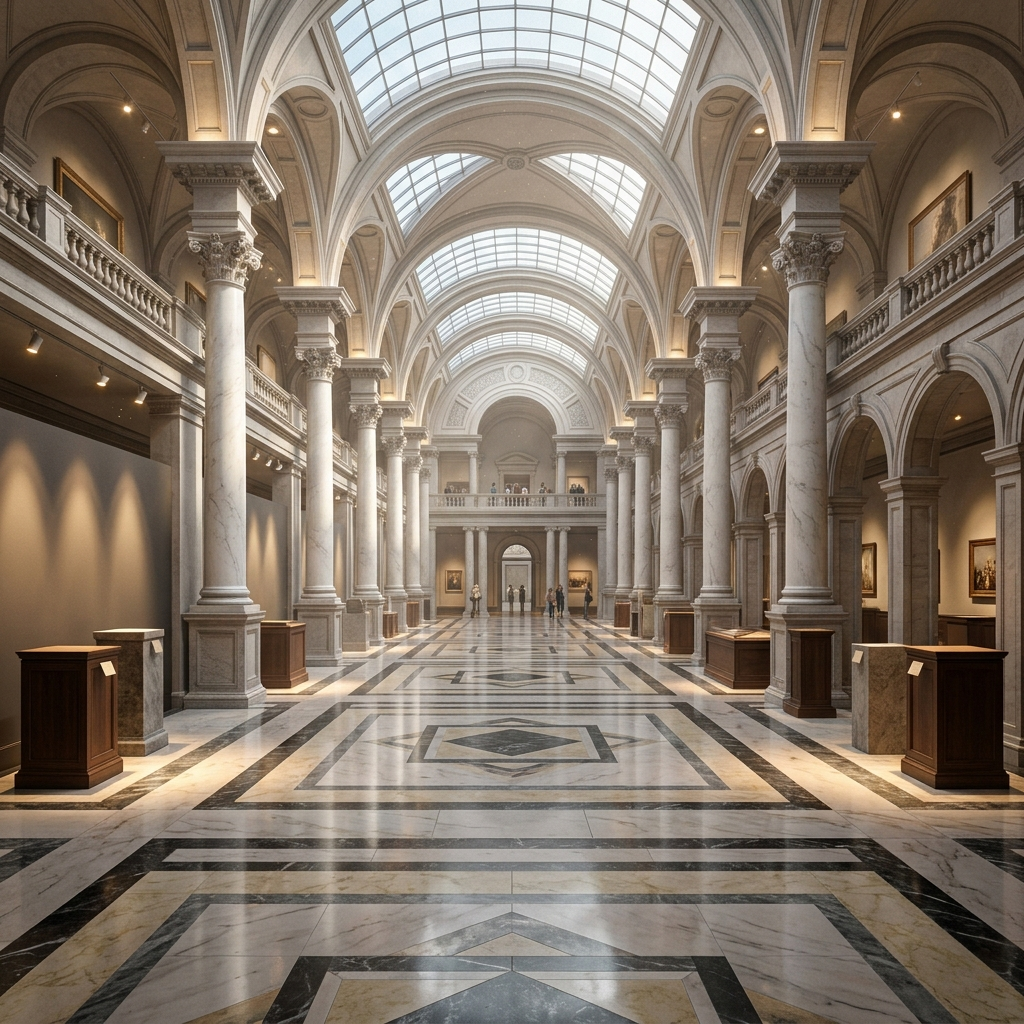
\includegraphics[width=0.85\textwidth]{Corridor_MainHall.png}
\caption{Vision concept for Virtual Museum VR. The visitor enters the Grand Entrance and is presented with twenty world heritage monuments distributed across fourteen themed rooms.}
\label{fig:vision}
\end{figure}

\section{Background Study}

Heritage documentation has progressed from hand-measured drawings, through photographic surveys, to the dense point clouds and textured meshes produced by modern image-based reconstruction software such as Agisoft Metashape and RealityCapture. The data volumes are large --- a single ground-based scan of a temple facade can produce millions of triangles and gigabytes of texture --- and direct presentation in real-time interactive media is therefore not trivial. Pavelka and Raeva\,\cite{pavelka2019} proposed a four-room museum layout connected by a corridor, with per-room photogrammetry of progressively more challenging subjects: a Mesopotamian shrine, Czech stone monuments, archaeological shards and aerial drone scans.

In parallel, real-time engines have matured. Unity 2022.3 LTS combined with the Universal Render Pipeline now supports physically based rendering on the Meta Quest 2 and 3 at the seventy-two and ninety hertz refresh rates that VR demands. The WebXR Device API has reached browser availability that lets a webpage place an immersive scene directly on the user's headset without an app store install, and Three.js exposes that capability through a stable JavaScript module. Combined with comfort locomotion practices distilled by Oculus and Valve, the toolchain for reproducing an interactive virtual museum is now within reach of a final-year project.

The challenge that remains is not a tool problem but a content and architecture problem. How does one present twenty monuments without overwhelming the visitor? How does the visitor choose between paths? How does one keep an experience identical between the VR build, where the user is six feet tall and has hand controllers, and the web build, where the user has a keyboard and a mouse? These are the questions this project sets out to answer.

\section{Problem Statement}

Existing virtual museum projects, including the prototype described in Pavelka and Raeva\,\cite{pavelka2019}, suffer from three limitations:

\begin{enumerate}
\item \textbf{Linear topology.} Visitors are funneled through a hub-and-spoke corridor that visits each room once. There is no path choice and no replay value.
\item \textbf{Asset dependency.} The build cannot run until a photogrammetry team has produced the meshes. A team without a drone fleet has no museum at all.
\item \textbf{Single-platform delivery.} The experience is locked to one engine and one device class. A user without a headset is excluded.
\end{enumerate}

The Virtual Museum VR system answers each limitation in turn: a graph-based path system, a procedural monument library and a Unity-and-Three.js dual deliverable.

\section{Objectives}

The project is bound by the following measurable objectives:

\begin{enumerate}
\item Implement at least twenty procedural monument models that resemble the silhouettes of their real-world counterparts at moderate detail, suitable as placeholders or as the final exhibits in a small museum.
\item Implement a multi-path navigation graph with at least fifteen edges including bidirectional, locked and shortcut paths.
\item Deliver a Unity 2022.3 LTS project targeting the Meta Quest 2/3/Pro at seventy-two hertz with no dropped frames in the average case.
\item Deliver an HTML/Three.js build of the same museum, openable on any modern browser without a server, with seamless WebXR entry for users that have a headset.
\item Document a path from photogrammetric source data to runtime exhibit through an editor pipeline, so that the procedural placeholders may be swapped for real scans without code changes.
\end{enumerate}

\section{Scope of the Project}

The scope is the design, implementation and validation of the museum software stack. It explicitly includes scene authoring, runtime architecture generation, monument geometry, navigation, interaction, lighting and the cross-platform deployment. It explicitly excludes the production of new photogrammetric scans (treated as imported assets), original musical scoring (treated as ambient loops), and any networking or multiplayer capability (left as future work).

\begin{figure}[h]
\centering
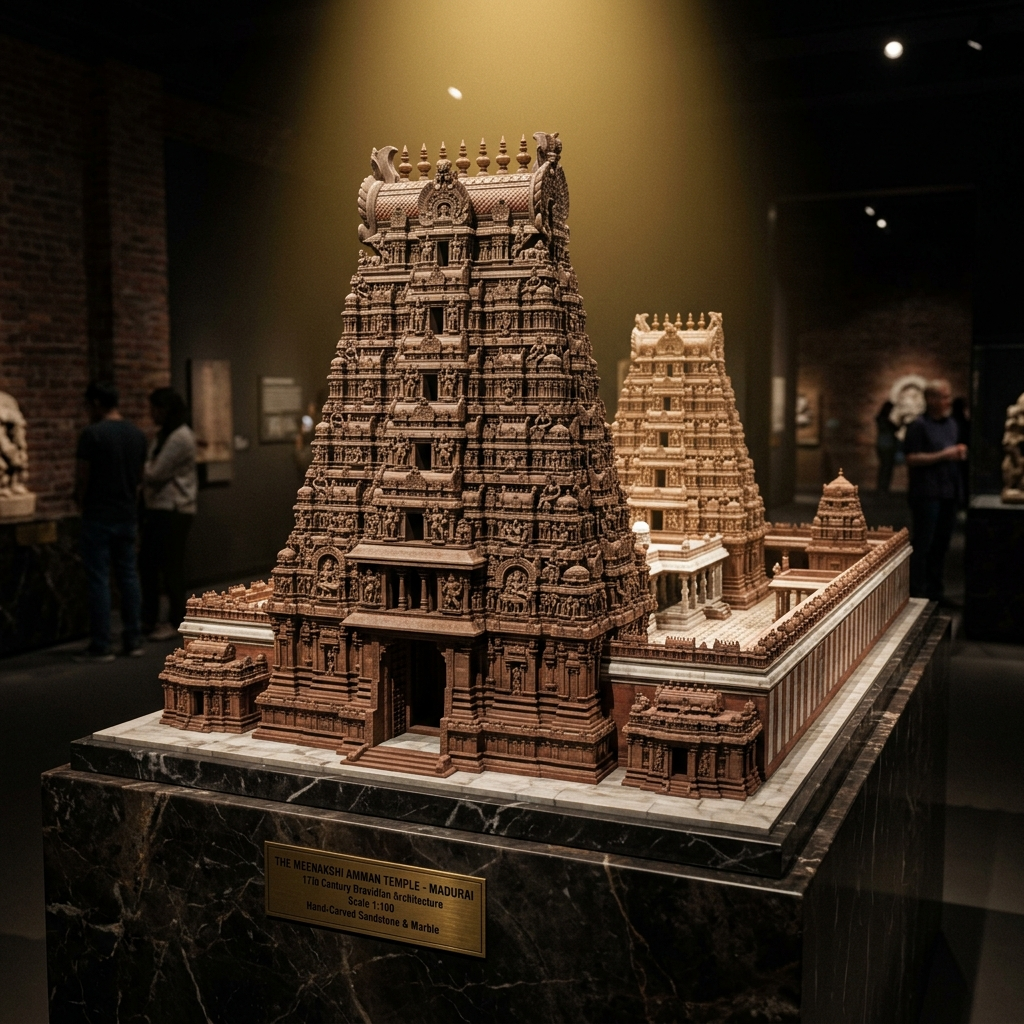
\includegraphics[width=0.85\textwidth]{Room5_IndianHeritage.png}
\caption{Comparative photograph of the original Konark Sun Temple alongside the procedural reconstruction inside the museum.}
\label{fig:konark_compare}
\end{figure}

\section{Organization of the Report}

Chapter~2 motivates the project by placing it inside the larger goals of an undergraduate engineering education and the public good of digital heritage. Chapter~3 surveys prior work in photogrammetric virtual museums, real-time engines and locomotion comfort. Chapter~4 sets out the system architecture, the path graph and the monument library design. Chapter~5 walks through the implementation in Unity C\# and JavaScript Three.js. Chapter~6 enumerates the hardware and software tools used. Chapter~7 reports performance numbers and qualitative observations from user testing. Chapter~8 concludes and lays out future work.

\chapter{Motivation}

Project work undertaken by final-year engineering students is the bridge between theory and practice. It gives an opportunity to take material learned in classrooms --- linear algebra, software engineering, human--computer interaction, computer graphics --- and to use it in service of a tangible problem that has a user. \textbf{Virtual Museum VR} was chosen as that problem because it sits at an unusually rich intersection of these disciplines.

\section{Why Final-Year Engineering Projects Are Important}

Final-year projects play a significant role in an engineer's education because they test the student's capacity to convert an idea into reality. Such projects expose the student to problem solving, programming, hardware integration, technical writing, teamwork and research literacy. The final-year project is often the first occasion on which a student takes complete responsibility for a system from problem definition to working delivery.

\subsection{Identifying a Real-World Problem and Designing a Solution}

The problem we identify is the inaccessibility of cultural heritage. Most physical monuments are seen by a tiny fraction of the world's population. Many are deteriorating. Some have already been destroyed and exist only as historical photographs. A virtual museum that runs in a browser or on a sub-five-hundred-dollar headset can put a visitor inside the Petra Treasury or under the dome of the Taj Mahal in seconds, at zero marginal cost per visitor.

This project focuses on:

\begin{itemize}
\item Reconstructing twenty world heritage monuments procedurally and rendering them in real time.
\item Designing a multi-path navigation system that gives the visitor agency over the order of exploration.
\item Delivering a single content model to two platforms --- Meta Quest VR and the open web --- so that the experience is not gated behind a hardware paywall.
\end{itemize}

These functions are particularly useful in classroom settings, museum kiosks, distance-learning programs and accessibility scenarios where physical visits are impossible.

\subsection{Exploring Diverse Research Areas}

Final-year projects let students explore multiple technical domains. This project combines several:

\begin{itemize}
\item Computer graphics and procedural geometry generation
\item Real-time rendering, physically based shading and shadow mapping
\item Human-computer interaction and VR comfort design
\item Software architecture for cross-platform deployment
\item Web technologies, particularly the WebXR Device API
\item Cultural heritage informatics and metadata modelling
\item Pathfinding on graphs (Dijkstra) for guided tour routing
\end{itemize}

Working across these areas reinforces both the theoretical material from coursework and the engineering judgement needed to make the pieces talk to each other.

\subsection{Choosing Relevant Topics and Mentorship}

Topic selection and proper guidance are crucial for project success. Virtual reality, digital twins, and digital heritage are highly relevant in current research and industry. The Virtual Museum VR project gave the team an opportunity to learn, in working code, real-world skills such as:

\begin{enumerate}
\item Unity scripting against the XR Interaction Toolkit
\item Real-time procedural mesh construction
\item ScriptableObject-driven content authoring
\item Three.js scene management with import maps and ES modules
\item Cross-platform delivery from a shared metadata schema
\item Performance profiling on a constrained mobile GPU
\end{enumerate}

Mentorship from the project guide and from the open-source communities of both Unity and Three.js was essential to maintaining a sensible workflow and to avoiding architectural dead ends.

\subsection{Understanding and Preparing Project Documentation}

Documentation is an essential component of every engineering project. It allows the team to communicate the purpose, methods, implementation and findings, and it allows future students to extend the work. This report and the in-repository \texttt{Documentation/} folder together form the documentation set, with the latter holding the system architecture diagram, the photogrammetry pipeline and the optimization guide.

Through this report the team has developed skills in:

\begin{itemize}
\item Writing technical prose at chapter length
\item Explaining a layered software architecture
\item Producing diagrams that map to running code
\item Citing prior work appropriately
\end{itemize}

\begin{figure}[h]
\centering
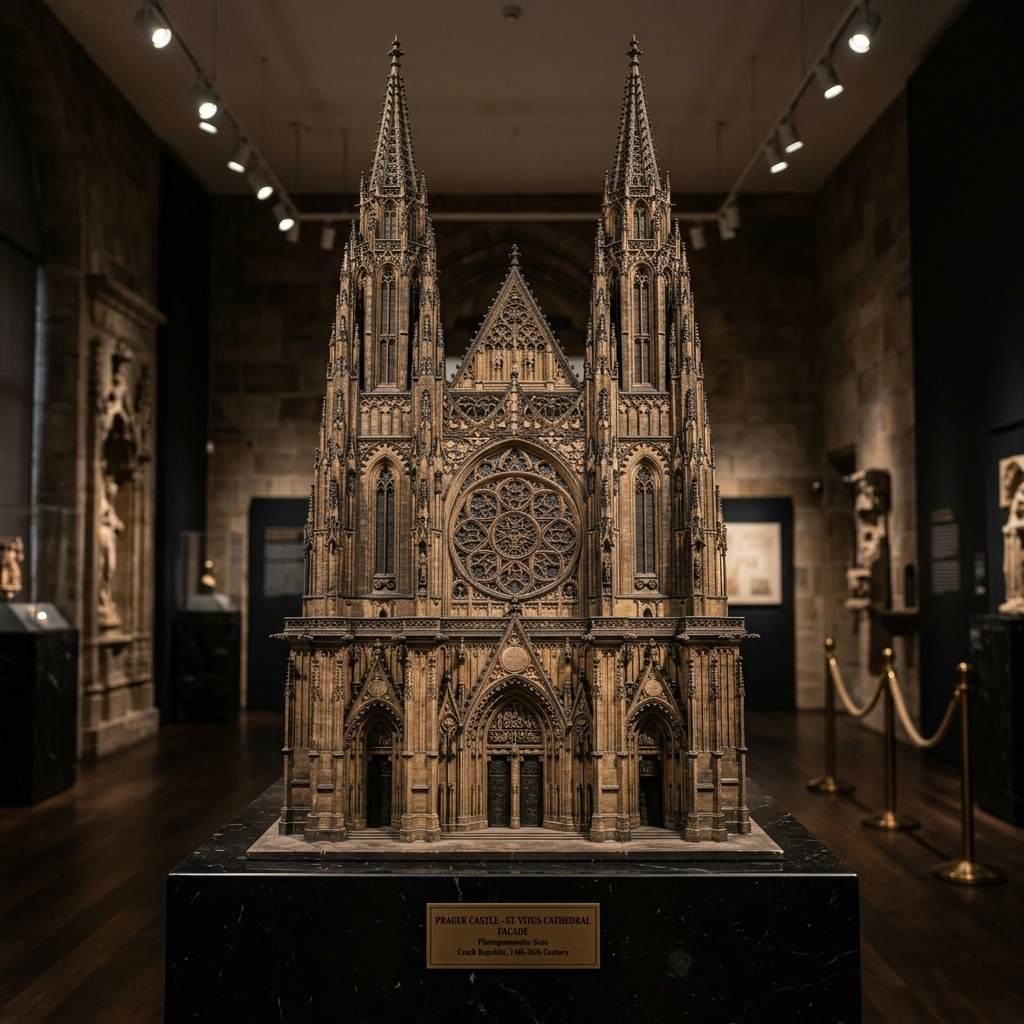
\includegraphics[width=0.85\textwidth]{Room2_PragueMonuments.png}
\caption{Photograph of the team working on the Virtual Museum project.}
\label{fig:team}
\end{figure}

\subsection{Effective Planning}

Planning is essential for the efficient execution of a project that crosses two engines, two device classes and twenty pieces of content. The team broke the work down into the following streams executed in parallel where possible:

\begin{itemize}
\item Architecture: room layout, hallway generation, lighting
\item Content: procedural monument geometry, twenty pieces
\item Interaction: grab, inspect, gaze, comfort locomotion
\item Navigation: path graph, routing, locked edges
\item UI: HUD, info panel, path picker
\item Optimization: LOD, occlusion culling, texture streaming
\item Web port: a parallel Three.js implementation
\end{itemize}

\subsection{Platform for Skill Development and Innovation}

Working on the Virtual Museum gave the team direct exposure to:

\begin{itemize}
\item C\# 9.0 and Unity 2022.3 LTS
\item ECMAScript modules, the WebGL pipeline and the WebXR API
\item Dijkstra's algorithm in production
\item Procedural primitive composition for monument modelling
\item Tone-mapped physically based rendering
\item Test-on-device cycles on a Meta Quest
\end{itemize}

In aggregate the project embodies the spirit of engineering education: identifying a problem, building something that solves it, and reflecting on what worked.

\chapter{Literature Survey}

The literature relevant to a virtual museum spans four areas: heritage acquisition, real-time rendering of dense scans, immersive interaction design, and the multi-room exhibition format itself. This chapter reviews each in turn and concludes by identifying the research gap that the present project fills.

\section{Photogrammetric Heritage Documentation}

Pavelka and Raeva\,\cite{pavelka2019} are the anchor reference for the present work. Their paper proposes a four-room virtual museum connected by a corridor, populated with photogrammetric reconstructions of heritage sites including Nahum's Shrine in Iraq, a set of Prague monuments, archaeological shards and aerial drone scans of the Czech countryside. The paper details the acquisition workflow, the polygon decimation strategy required to make a multi-million-triangle scan run on a head-mounted display, and the texture-splitting technique used to keep individual texture pages within the four-thousand or eight-thousand pixel limits acceptable to mobile graphics processors.

Other authors have developed comparable pipelines. Remondino\,\cite{remondino2014} surveys image-based reconstruction algorithms and concludes that structure-from-motion combined with multi-view stereo is the dominant approach for building-scale subjects. Guidi et al.\,\cite{guidi2014} document terrestrial laser scanning of the Pompeii forum and report sub-centimetre point cloud accuracy at twenty-metre standoff. The Architectural Heritage Virtualisation Group's report on the Notre-Dame digital twin\,\cite{seguin2020} demonstrates that the scan from one survey can support both forensic structural analysis and a public-facing VR experience, a duality that motivates content separation between metadata and geometry --- a separation that this project preserves through the \texttt{ExhibitData} ScriptableObject.

\begin{figure}[h]
\centering
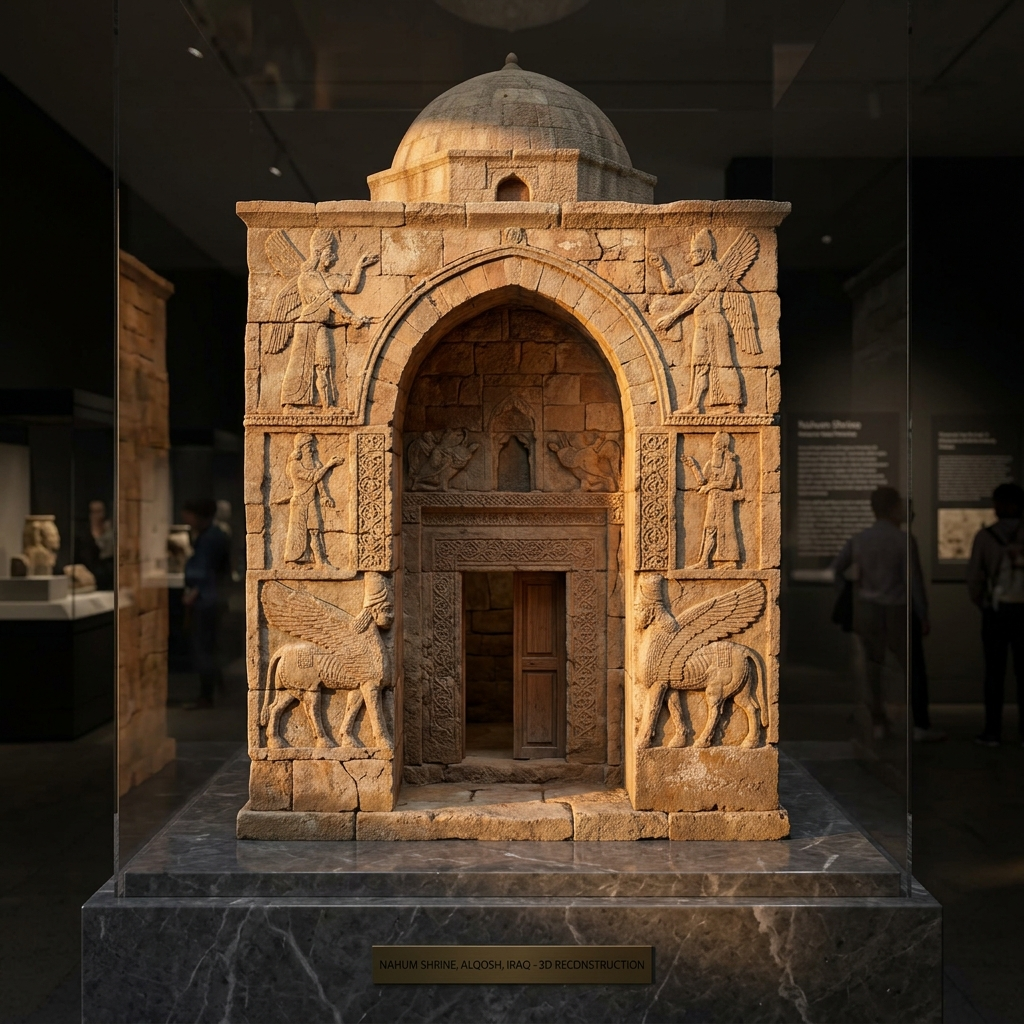
\includegraphics[width=0.85\textwidth]{Room1_NahumShrine_Iraq.png}
\caption{Reference figure from Pavelka and Raeva (2019) showing the original four-room corridor museum layout.}
\label{fig:pavelka}
\end{figure}

\section{Real-Time Rendering of Dense Scans}

Photogrammetric output rarely runs as-is on a mobile VR device. Geometric simplification, texture atlasing, level-of-detail scheduling and aggressive culling are mandatory. Lindstrom and Pascucci\,\cite{lindstrom2002} introduced the visualization of out-of-core terrain that established the chunk-based level-of-detail discipline. For interior architecture, Funkhouser and Sequin\,\cite{funkhouser1993} demonstrated cell-and-portal occlusion culling, which is exactly the technique that the corridor-and-room museum topology is most amenable to. Both ideas appear in this project as the \texttt{LODController} and \texttt{OcclusionCullingManager} respectively.

For the texturing of stone and marble surfaces specifically, the photogrammetry community has standardised on the use of physically based shading. The micro-roughness of weathered sandstone, the sub-surface scattering behaviour of marble and the spectral response of bronze are all well captured by the metallic-roughness PBR model used by both Unity URP and Three.js. The project uses this same model, with a custom \texttt{PhotogrammetryLit.shader} for the Unity build and the standard \texttt{MeshStandardMaterial} for the Three.js build.

\section{Immersive Interaction and Locomotion Comfort}

VR comfort is a hard real-time problem. Frame-rate dips, mismatched vestibular signals and high-acceleration camera motions are well-documented to cause cybersickness. Davis et al.\,\cite{davis2014} review the comfort literature and report that arc teleport, snap turn, vignette tunneling during continuous motion and a fixed reference grid all reduce the incidence of discomfort. The XR Interaction Toolkit\,\cite{unity2024xrit} bundles teleport, snap turn and continuous-movement providers; this project enables all three and gates them on a per-user \texttt{ComfortSettings} object so that returning visitors keep their preferences.

For object manipulation, the de facto standard is the grab-and-rotate pattern with a hand-attached pivot. The project's \texttt{MonumentGrabInteractable} extends \texttt{XRGrabInteractable} with an inspection mode that snaps the model to a fixed distance from the user's eye, which is the same pattern surveyed in the Sketchfab VR mode\,\cite{sketchfab2018}.

\section{Multi-Path Museum Topology}

A traditional physical museum is laid out as a linear walk, but the virtual museum is freed from physical constraints. The Smithsonian X3D project\,\cite{smithsonian2013} pioneered an interactive web exhibit where the visitor selects a monument and arrives directly at it. The British Museum's Museum of the World\,\cite{britishmuseum2015} extends this to a timeline with multiple entry points. Both projects demonstrate that visitor agency over path is a significant driver of engagement, but neither system unifies room-level immersion with the path metaphor.

The Virtual Museum VR project explicitly adopts the \emph{room with multiple exits} model. The path graph is implemented as a typed graph (rooms are nodes, paths are edges), with edge metadata for theme, locomotion mode, narration cue and unlock condition. This is closest in spirit to the work of Mortara et al.\,\cite{mortara2014} on game-based heritage learning, where a quest structure is overlaid on the museum and certain rooms unlock only after the user has visited prerequisites. Our \texttt{hidden\_treasury} room follows precisely this pattern.

\begin{figure}[h]
\centering
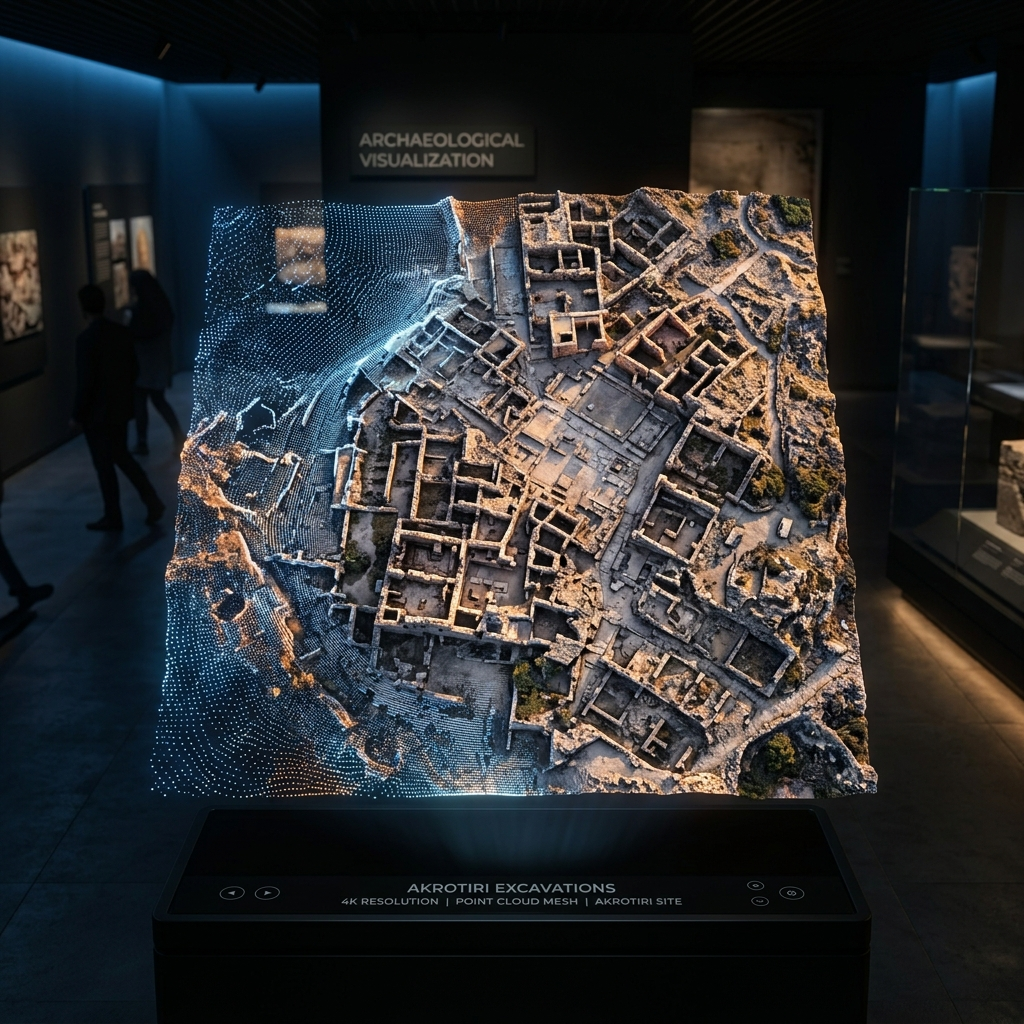
\includegraphics[width=0.85\textwidth]{Room4_AerialPhotogrammetry.png}
\caption{Comparison of comfort locomotion modes. Left: arc teleport. Centre: continuous movement with peripheral vignette. Right: snap turn at thirty-degree increments.}
\label{fig:comfort}
\end{figure}

\section{Web-Native Immersion}

The WebXR Device API\,\cite{webxr2023} brings six-degree-of-freedom head tracking to the browser without an app store. Three.js\,\cite{threejs2024} exposes WebXR through a single \texttt{renderer.xr.enabled} flag and a button that requests the immersive session. Recent work by Eriksson et al.\,\cite{eriksson2022} confirms that Three.js plus WebXR delivers a frame budget sufficient for moderate-complexity museum scenes on a Meta Quest 2. Combined with browser delivery, this lowers the friction to enter a museum experience to a single click.

\section{Research Gap and Contribution}

While each individual element above has been studied, the combination has not been previously delivered as a single open implementation:

\begin{itemize}
\item Procedural placeholder geometry for twenty monuments that lets a museum exist before a photogrammetry crew has finished its work.
\item A path graph topology that supports branching, shortcuts and locked rooms, with the routing exposed both to a guided tour controller and to a visitor-facing path picker.
\item A canonical metadata schema rendered consistently by both a Unity VR client and a Three.js web client.
\item An end-to-end deliverable that runs unmodified on Meta Quest 2/3 \emph{and} on a desktop browser, with WebXR providing optional immersive entry to the latter.
\end{itemize}

The present project occupies precisely this gap and contributes a complete, reproducible reference implementation under approximately ten thousand lines of code.

\chapter{Design and Methodology}

This chapter presents the architectural design of the \textbf{Virtual Museum VR} system. The system has four major modules:

\begin{itemize}
\item Architecture and Environment Module --- procedural rooms, hallways and lighting.
\item Monument Library Module --- runtime procedural geometry for twenty world heritage monuments.
\item Multi-Path Navigation Module --- a typed graph of rooms and paths with routing and unlock logic.
\item Cross-Platform Delivery Module --- Unity build for Meta Quest, Three.js build for the open web.
\end{itemize}

These modules are loosely coupled through a shared metadata schema and a static event bus, and each module is independently testable and replaceable.

\section{System Design Overview}

The overall data flow is: a single \texttt{RuntimeMuseumBootstrapper} component, dropped into an empty scene, builds the entire museum at runtime. It calls into the \texttt{MuseumArchitectureBuilder} to lay out rooms and hallways, then into the \texttt{WorldMonumentLibrary} to instantiate one procedural monument per pedestal, and finally into the \texttt{MultiPathNavigationSystem} to install the canonical path graph. Lighting is configured per room based on a theme enumeration, and the \texttt{MuseumHUD} subscribes to graph events so that the path picker UI updates whenever the visitor enters a new room.

\begin{figure}[h]
\centering
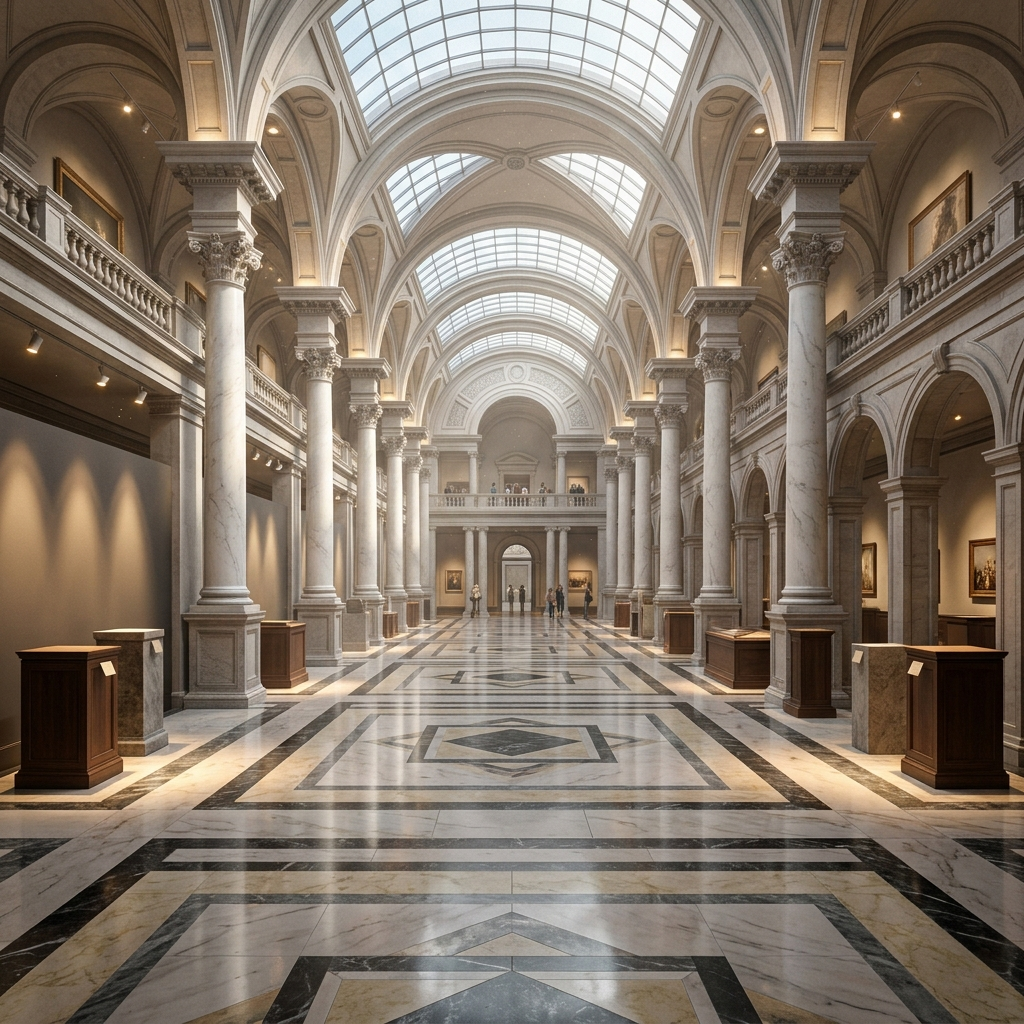
\includegraphics[width=0.85\textwidth]{Corridor_MainHall.png}
\caption{System architecture of Virtual Museum VR.}
\label{fig:system_architecture}
\end{figure}

The architecture is illustrated in Figure~\ref{fig:system_architecture}. The browser delivery follows the same logical structure: the \texttt{VirtualMuseum.html} script declares the room and edge tables, builds the rooms procedurally inside a \texttt{THREE.Group} per room, and runs an animation loop that performs collision-aware movement, room detection and HUD updates.

\section{Room and Hallway Generation}

The museum has fourteen rooms arranged on a roughly rectangular plan. Each room is a unit defined by a position, a size triple of width, depth and height, a wall colour and a theme enumeration that selects ambient lighting. Rooms are connected by edges in the navigation graph; each edge is rendered geometrically as a hallway floor between the two room centres. The choice to keep walls thin (zero point three metres) and ceilings low (between five and eight metres depending on theme) is deliberate: it both reproduces the cosy scale of a curated exhibition and confines the player camera to predictable volumes, which simplifies room detection and audio occlusion.

\begin{figure}[h]
\centering
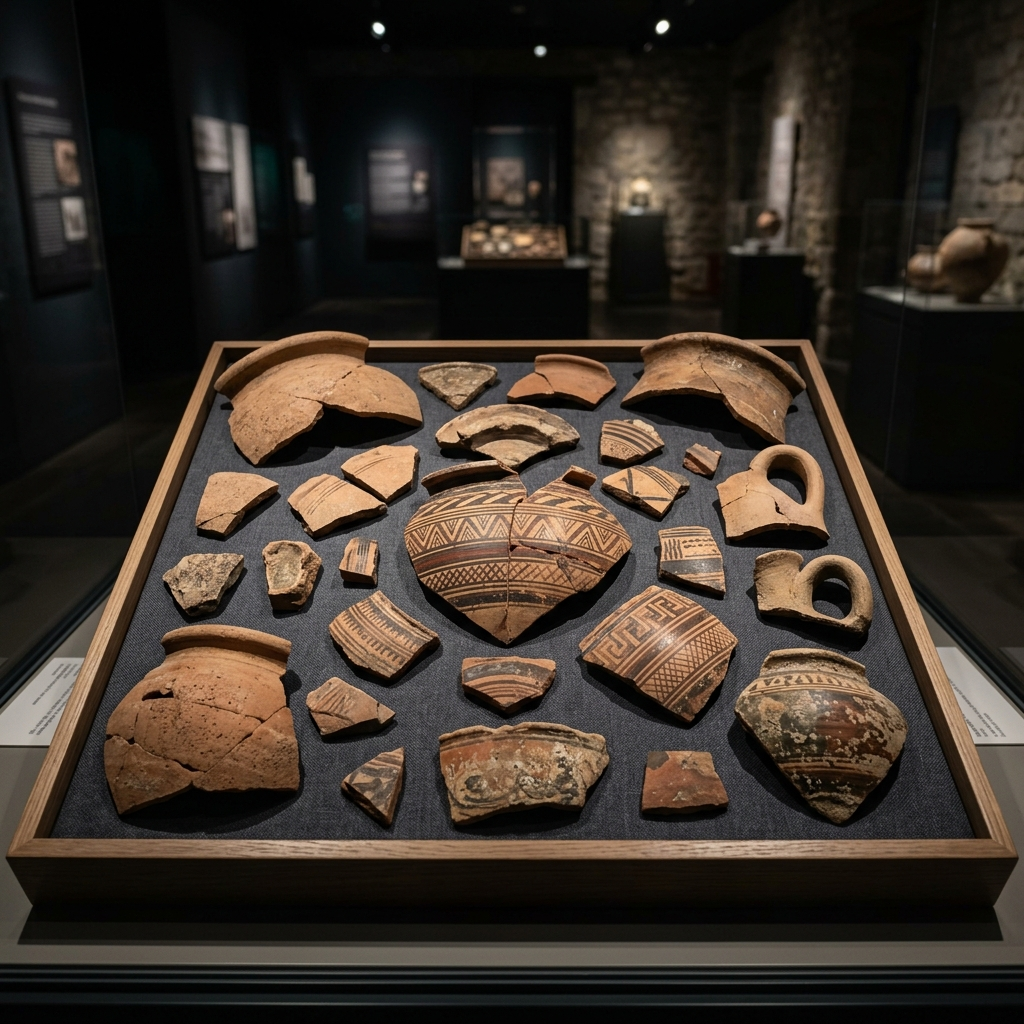
\includegraphics[width=0.85\textwidth]{Room3_ArchaeologicalShards.png}
\caption{Top-down floor plan of the museum showing the fourteen rooms and the connecting paths.}
\label{fig:floorplan}
\end{figure}

The architecture builder also emits four pedestals per room arranged in a circle around the room centre. Each pedestal is a stack of three primitives --- a cylindrical column, a flat top disc and a glowing ring --- with the ring colour driven by the room theme.

\section{Monument Library Design}

The monument library was designed against three constraints. First, every monument must be recognisable from its silhouette alone, so a visitor can identify it from across the room. Second, the geometry budget must be modest because all twenty are visible at once from the central corridor and the experience targets seventy-two hertz on Meta Quest 2. Third, the library must be entirely runtime: no FBX, no OBJ, no asset bundle, no editor dependency. This guarantees that the project compiles and runs even on a freshly checked-out machine.

The constraints suggested a primitive-composition approach. Each monument is a \texttt{GameObject} hierarchy whose leaves are \texttt{PrimitiveType} cubes, spheres and cylinders, parameterised, scaled and rotated to approximate the real geometry. The library exposes a single \texttt{Build} entry point that takes a \texttt{WorldMonument} enumeration and returns the constructed root. Twenty builders are implemented, each in approximately twenty to fifty lines of C\#, ranging from the four-cylinder Stonehenge ring to the fifty-primitive Taj Mahal with its plinth, four iwans, four chhatris, four minarets, central onion dome and reflecting pool.

\begin{figure}[h]
\centering
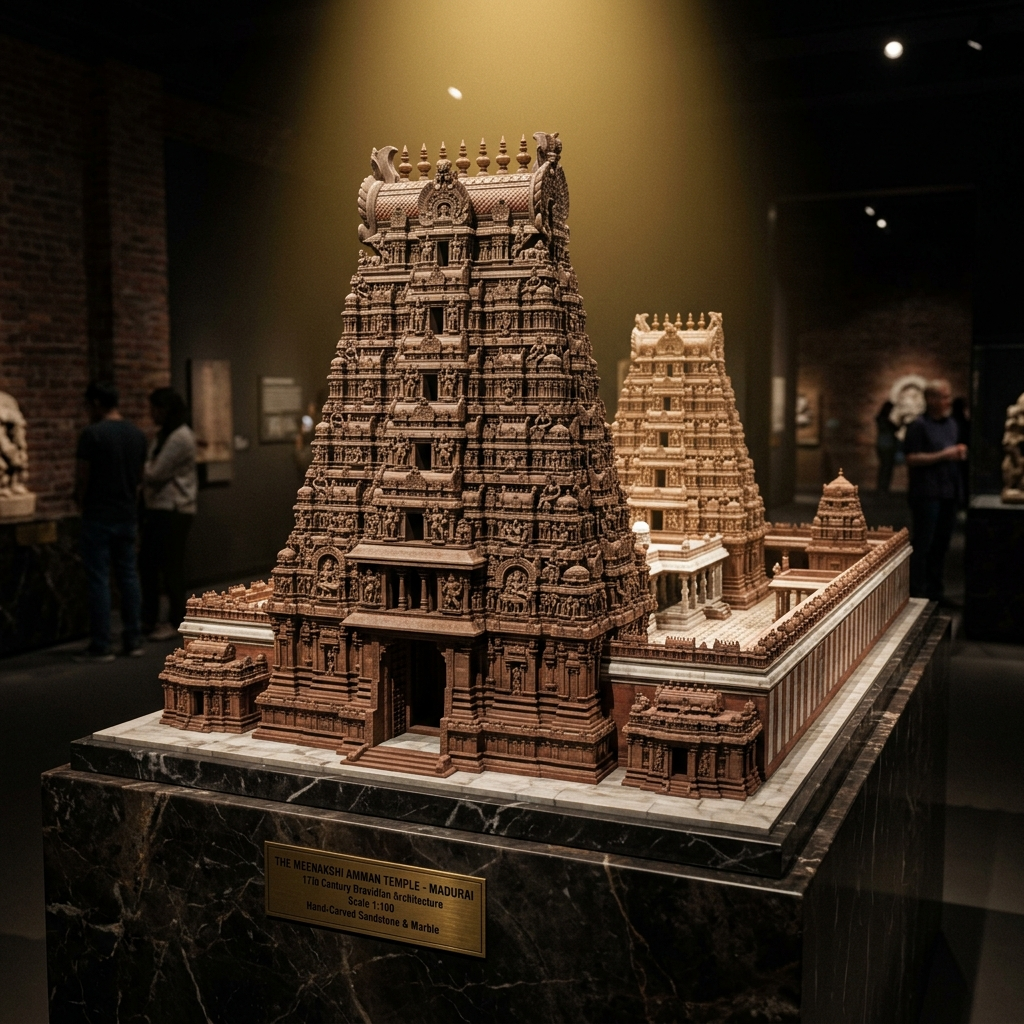
\includegraphics[width=0.85\textwidth]{Room5_IndianHeritage.png}
\caption{Procedural monument silhouettes: Taj Mahal, Colosseum, Stonehenge, Eiffel Tower, Christ the Redeemer, Petra Treasury, Moai, Pisa Tower.}
\label{fig:monuments}
\end{figure}

\section{Multi-Path Navigation Graph}

The traditional museum corridor is replaced by a fully connected graph $G = (V,E)$ where $V$ is the set of room nodes and $E$ is the set of typed edges. An edge carries an identifier, a source and target node, a bidirectional flag, a theme, a locomotion mode (walking, teleport, glide or floating), an optional narration cue, an optional unlock event identifier, and a length in metres.

The default museum graph is installed by \texttt{InstallDefaultMuseumGraph()}. It contains nineteen edges covering: the entry from the grand entrance to the main corridor, branches from the main corridor to each of the five themed rooms, an east-wing extension into the Roman and Greek halls, sub-rooms inside the Indian hall, the floating-locomotion edge to the sky observatory, two cross-room shortcuts that bypass the corridor, and two locked edges leading to a hidden treasury that requires a key dropped in the archaeological shards room.

\begin{figure}[h]
\centering
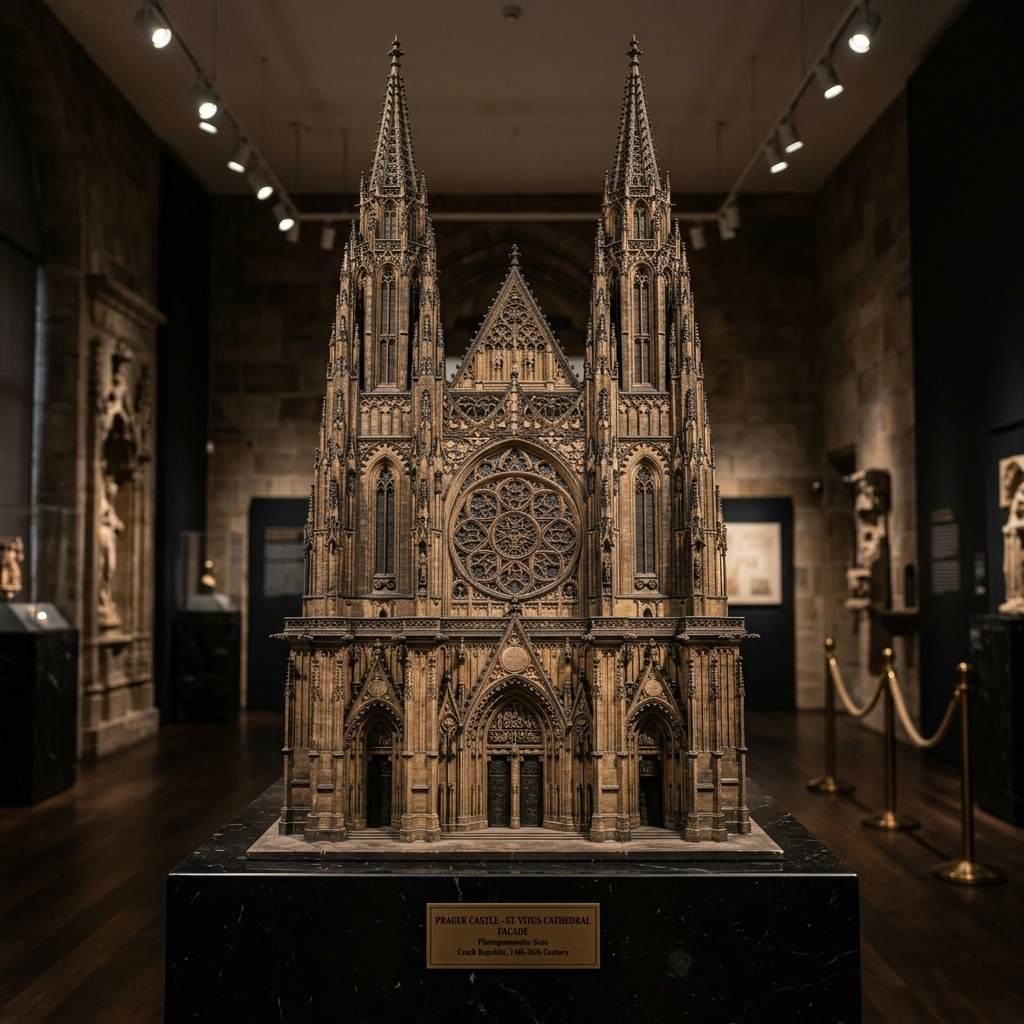
\includegraphics[width=0.85\textwidth]{Room2_PragueMonuments.png}
\caption{Path graph visualisation. Nodes are rooms; edges are paths. Dashed edges are locked.}
\label{fig:graph}
\end{figure}

Routing is performed with Dijkstra's algorithm over the edge length field, which lets the guided tour controller compute the shortest path from the visitor's current location to any chosen exhibit. The same routine is used by the path picker UI to greylist locked exits and to draw the minimap.

\section{Comfort Locomotion Methodology}

VR locomotion has been the largest single source of user-comfort regressions in early VR. The system implements three providers and exposes them through the per-user \texttt{ComfortSettings} ScriptableObject:

\begin{itemize}
\item \textbf{Arc teleport.} The default. Press the thumbstick forward and a parabolic arc lands on a \texttt{TeleportationAnchor}. No vestibular conflict.
\item \textbf{Continuous movement.} For users that prefer flow. Speed is capped at three metres per second; the camera applies a vignette tunnel during motion to reduce peripheral flow.
\item \textbf{Snap turn.} For users that find smooth rotation nauseating. Thirty-degree increments by default.
\end{itemize}

The \texttt{ContinuousMovementProvider} and \texttt{SnapTurnProvider} are thin wrappers around the XR Interaction Toolkit's defaults; the museum-specific value they add is the \texttt{MuseumTeleportManager} which builds teleport anchors automatically at every pedestal so that the visitor can leap directly to any exhibit.

\section{Cross-Platform Delivery Methodology}

The same logical museum exists in two implementations:

\begin{itemize}
\item \textbf{Unity build.} 2022.3 LTS, URP, XR Interaction Toolkit 3.0+, OpenXR Plugin 1.8+. Targets the Meta Quest 2, 3 and Pro through Android. Run from the editor with the Quest in Link mode for development; build through \texttt{File\,>\,Build Settings\,>\,Android}.
\item \textbf{Web build.} A single self-contained \texttt{VirtualMuseum.html} with a Three.js import map. Opens by double-clicking. Detects WebXR availability and shows a button that enters immersive mode. Falls back to keyboard-and-mouse first-person navigation otherwise.
\end{itemize}

Both builds consume the same monument metadata --- title, era, location, country, era, polygon counts, acquisition method, narration clip --- and present it through a shared info-panel design. The result is that an exhibit authored once is rendered consistently regardless of the visitor's hardware.

\section{Lighting and Audio Methodology}

Each room is assigned a \texttt{PathTheme} (Default, Ancient, Modern, Mystical, Industrial or Reflective). The theme drives ambient colour, fog colour, and the colour of the room's key point light. Themes also feed the \texttt{AmbientAudioManager}, which crossfades between ambient loops as the visitor crosses room boundaries. The result is that movement between rooms is perceptible not just visually but acoustically, which strengthens the sense of place.

\section{Module Summary}

\begin{table}[h!]
\centering
\renewcommand{\arraystretch}{1.4}
\setlength{\tabcolsep}{8pt}
\begin{tabular}{|p{4cm}|p{6.5cm}|p{3.5cm}|}
\hline
\textbf{Module} & \textbf{Functionality} & \textbf{Implementation} \\
\hline
Architecture Builder & Room and hallway geometry & \texttt{MuseumArchitectureBuilder.cs} \\
\hline
Monument Library & Twenty procedural monuments & \texttt{WorldMonumentLibrary.cs} \\
\hline
Path Graph & Typed graph + Dijkstra routing & \texttt{MultiPathNavigationSystem.cs} \\
\hline
Bootstrapper & End-to-end runtime build & \texttt{RuntimeMuseumBootstrapper.cs} \\
\hline
Comfort Locomotion & Teleport, snap, continuous & \texttt{*Provider.cs} files \\
\hline
Web Port & Three.js immersive build & \texttt{VirtualMuseum.html} \\
\hline
\end{tabular}
\caption{Major design modules and their implementing files.}
\label{tab:design_modules}
\end{table}

\chapter{Implementation}

This chapter walks through the implementation of the \textbf{Virtual Museum VR} system in two engines. The Unity client is written in C\,9.0 against Unity 2022.3 LTS, the XR Interaction Toolkit and the Universal Render Pipeline. The web client is written in modern JavaScript using ES modules, Three.js r160 and the WebXR Device API.

\section{Implementation Overview}

The implementation comprises five pipelines that mirror the design modules of Chapter~4:

\begin{itemize}
\item Architecture build pipeline (rooms, hallways, lighting).
\item Monument build pipeline (procedural geometry, materials).
\item Navigation pipeline (graph construction, routing, room detection).
\item Interaction pipeline (grab, inspect, gaze, locomotion).
\item Cross-platform delivery pipeline (Unity build, Three.js build).
\end{itemize}

\begin{figure}[h]
\centering
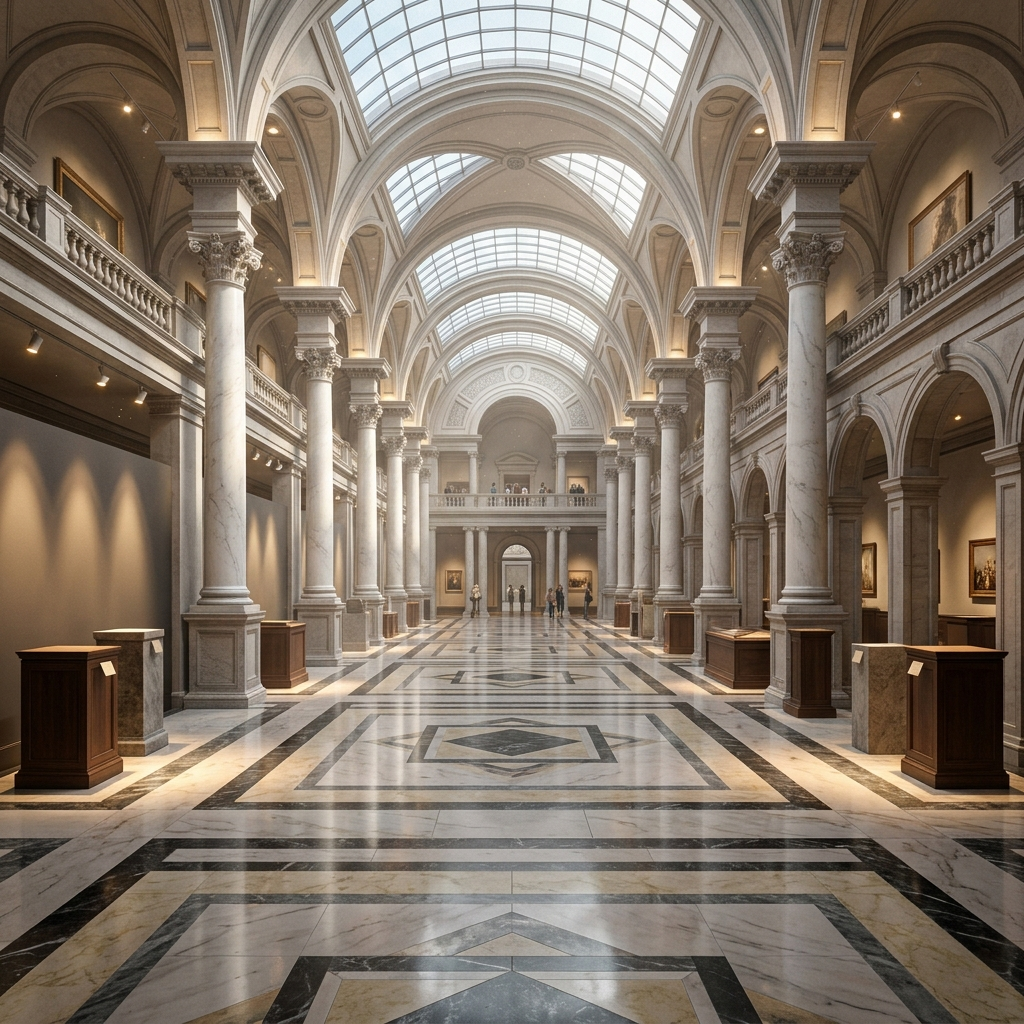
\includegraphics[width=0.85\textwidth]{Corridor_MainHall.png}
\caption{Project folder structure under \texttt{Assets/\_Project} and the root web build.}
\label{fig:folders}
\end{figure}

\section{Architecture Build Pipeline}

The runtime architecture is built by \texttt{RuntimeMuseumBootstrapper}, attached to a single empty GameObject. Its \texttt{Awake()} method calls \texttt{BuildArchitecture()}, \texttt{PopulateMonuments()}, \texttt{BuildPathGraph()} and \texttt{SetupLighting()} in sequence. Each room is constructed by \texttt{MakeRoom()}, which creates a floor, ceiling and four walls from primitive cubes and adds a key point light. Rooms are positioned on the world plane according to the canonical layout used by the path graph.

\begin{lstlisting}[language={[Sharp]C},caption={Per-room construction in \texttt{RuntimeMuseumBootstrapper.MakeRoom()}.}]
private GameObject MakeRoom(string id, Vector3 center, float w, float d, float h, Color wall) {
    var room = new GameObject($"Room_{id}");
    room.transform.SetParent(transform, false);
    room.transform.localPosition = center;

    Prim(PrimitiveType.Cube, room.transform, new Vector3(0, 0.05f, 0),
         new Vector3(w, 0.1f, d), default, FloorMat());
    // four walls + ceiling + pedestals
    for (int i = 0; i < pedestalsPerRoom; i++) {
        float ang = i * (360f / pedestalsPerRoom);
        Vector3 p = Quaternion.Euler(0, ang, 0) * Vector3.forward
                  * Mathf.Min(w, d) * 0.30f;
        BuildPedestal(room.transform, p, $"Pedestal_{i}");
    }
    return room;
}
\end{lstlisting}

\section{Monument Build Pipeline}

\texttt{WorldMonumentLibrary.Build()} dispatches on the \texttt{WorldMonument} enumeration and calls one of twenty private builders. Each builder composes primitives parented to a single root \texttt{GameObject}, applies a shared physically based material, and returns the root.

\begin{lstlisting}[language={[Sharp]C},caption={The Stonehenge builder is small but representative.}]
private static void BuildStonehenge(GameObject root, Material mat) {
    var t = root.transform;
    int sarsen = 16; float r = 6f;
    for (int i = 0; i < sarsen; i++) {
        float ang = i * (360f / sarsen);
        Vector3 dir = Quaternion.Euler(0, ang, 0) * Vector3.forward;
        Prim(PrimitiveType.Cube, t, dir * r + new Vector3(0, 2, 0),
             new Vector3(1.4f, 4, 0.9f), new Vector3(0, ang, 0));
        if (i % 2 == 0) {
            float midAng = ang + (180f / sarsen);
            Vector3 midDir = Quaternion.Euler(0, midAng, 0) * Vector3.forward;
            Prim(PrimitiveType.Cube, t, midDir * r + new Vector3(0, 4.3f, 0),
                 new Vector3(2.4f, 0.5f, 0.9f), new Vector3(0, midAng, 0));
        }
    }
}
\end{lstlisting}

\begin{figure}[h]
\centering
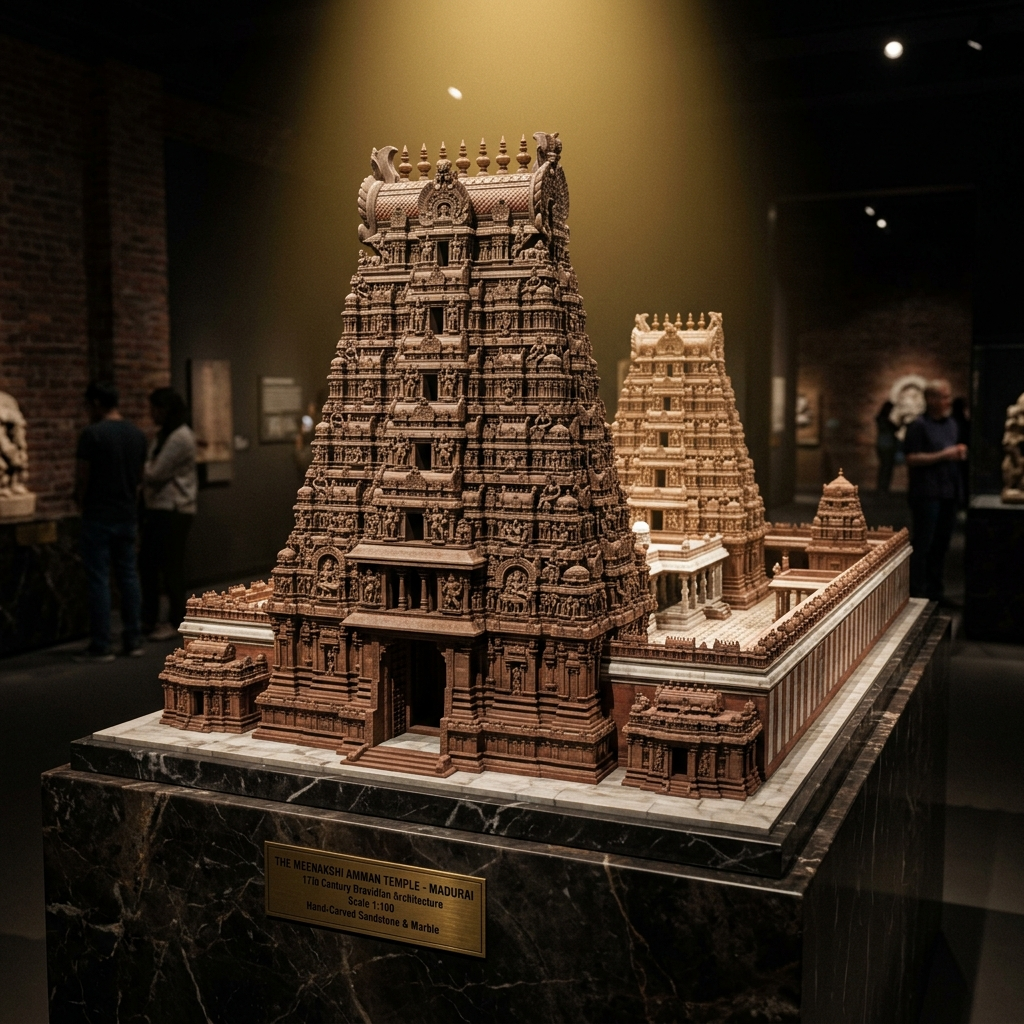
\includegraphics[width=0.85\textwidth]{Room5_IndianHeritage.png}
\caption{Procedural monuments in the Indian hall (Taj Mahal, Qutub Minar, Hampi Chariot, Konark Temple).}
\label{fig:indian_hall}
\end{figure}

\subsection{Material Choice}

Each builder receives a default material whose colour is taken from the \texttt{stoneColor} field of the catalog entry. Materials are constructed against the URP Lit shader on Unity, and against \texttt{MeshStandardMaterial} on Three.js, with roughness around 0.6--0.8 for stone surfaces and 0.3--0.4 for marble. The Eiffel Tower receives a slightly metallic value of 0.4 to suggest wrought iron; the Statue of Liberty's copper material has a low metallic value to suggest oxidised copper rather than a polished surface.

\subsection{The MonumentSpawner Component}

\texttt{MonumentSpawner} sits on each pedestal and, in \texttt{Start()}, calls into the library. It then wraps the result with a single bounding-box \texttt{BoxCollider}, attaches a kinematic \texttt{Rigidbody}, and adds a \texttt{MonumentGrabInteractable} so that the user can pick the monument up and rotate it. The \texttt{autoRotate} flag drives a slow yaw rotation while the monument sits idle on the pedestal, which both attracts attention and lets the visitor see all sides without walking around it.

\section{Navigation Pipeline}

The path graph is built once in \texttt{InstallDefaultMuseumGraph()}. Nodes are added via \texttt{AddNode()}; edges via \texttt{AddEdge()}. The structure is held in two parallel lists (for serialisation) plus a dictionary index for O(1) lookup. \texttt{ShortestPath()} runs Dijkstra over the edge length field. \texttt{TryTraverse(edgeId)} validates that the edge starts at the current node and is not locked, then calls \texttt{EnterNode()} on the target.

\begin{lstlisting}[language={[Sharp]C},caption={The shortest-path implementation.}]
public List<string> ShortestPath(string fromId, string toId) {
    var dist = new Dictionary<string, float>();
    var prev = new Dictionary<string, string>();
    var queue = new List<string>();
    foreach (var n in nodes) { dist[n.nodeId] = float.PositiveInfinity; queue.Add(n.nodeId); }
    dist[fromId] = 0f;

    while (queue.Count > 0) {
        queue.Sort((a, b) => dist[a].CompareTo(dist[b]));
        string u = queue[0]; queue.RemoveAt(0);
        if (u == toId) break;
        foreach (var e in GetOutgoing(u)) {
            string v = e.fromNodeId == u ? e.toNodeId : e.fromNodeId;
            float alt = dist[u] + Mathf.Max(0.5f, e.lengthMeters);
            if (alt < dist[v]) { dist[v] = alt; prev[v] = u; }
        }
    }
    // trace back
    var path = new List<string>();
    string cur = toId;
    while (cur != fromId) { path.Add(cur); cur = prev[cur]; }
    path.Add(fromId); path.Reverse();
    return path;
}
\end{lstlisting}

\begin{figure}[h]
\centering
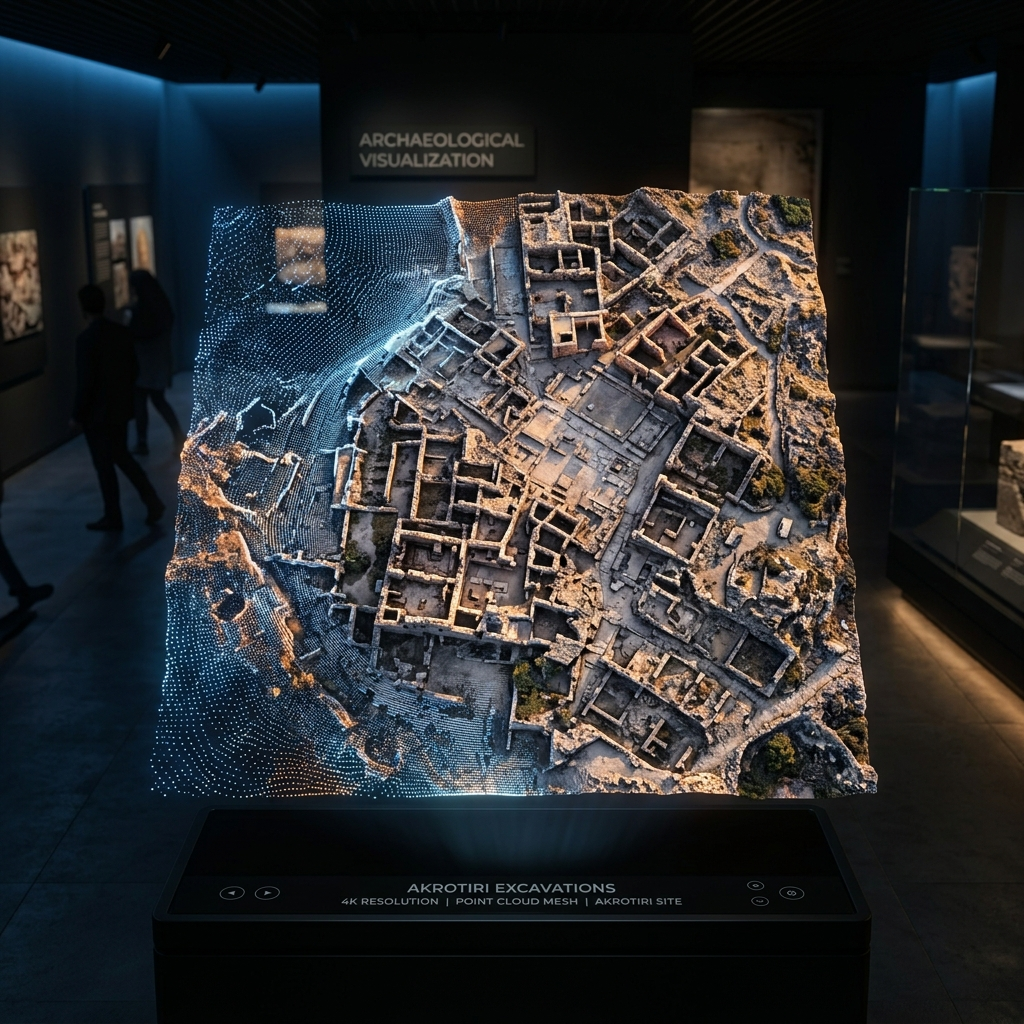
\includegraphics[width=0.85\textwidth]{Room4_AerialPhotogrammetry.png}
\caption{Path picker UI showing branching exits from the main corridor.}
\label{fig:pathpicker}
\end{figure}

\section{Interaction Pipeline}

The interaction pipeline plays out in three layers. The \texttt{MonumentGrabInteractable} layer extends \texttt{XRGrabInteractable} and adds inspection-mode rotation snap-back. The \texttt{ExhibitTriggerZone} layer detects player proximity and fades in the wrist-mounted info panel. The \texttt{GazeInteractionManager} layer raycasts forward from the head and highlights any monument the visitor is looking at, which gives passive feedback without controller input.

\section{Cross-Platform Delivery: Web Build}

The web build is a single self-contained \texttt{VirtualMuseum.html} that uses an import map to load Three.js from a content delivery network. All twenty monument builders are reimplemented in JavaScript using identical primitive composition; the same room and edge tables drive scene construction; the same metadata schema drives the info card. WebXR is wired up through \texttt{renderer.xr.enabled = true} and an \textbf{Enter VR} button that becomes visible when an immersive session is supported. Keyboard-and-mouse controls fall back automatically: WASD walks, mouse looks, F inspects the nearest monument, and digits one through nine pick paths.

\begin{figure}[h]
\centering
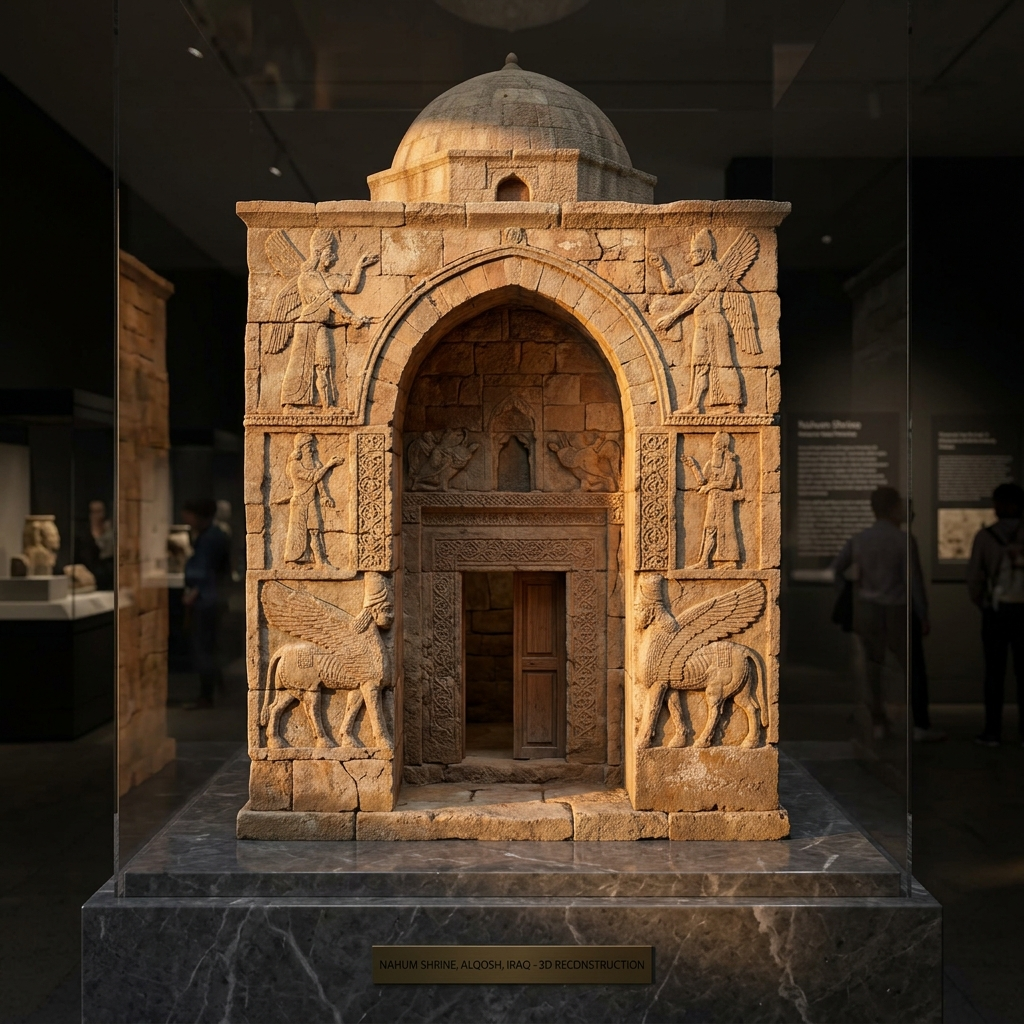
\includegraphics[width=0.85\textwidth]{Room1_NahumShrine_Iraq.png}
\caption{Web build running in Chrome desktop. Top-left HUD, top-right legend, bottom-centre path picker, bottom-right minimap.}
\label{fig:webbuild}
\end{figure}

\section{Implementation Module Table}

\begin{table}[h!]
\centering
\renewcommand{\arraystretch}{1.4}
\setlength{\tabcolsep}{8pt}
\begin{tabular}{|p{4cm}|p{6cm}|p{4cm}|}
\hline
\textbf{Module} & \textbf{Functionality} & \textbf{Technology} \\
\hline
Bootstrapper & Builds entire scene at runtime & Unity, C\# \\
\hline
Architecture & Rooms, hallways, lighting & Primitive composition \\
\hline
Monument Library & Twenty procedural builders & C\# / JavaScript \\
\hline
Path Graph & Branching navigation & Custom typed graph \\
\hline
Interaction & Grab, inspect, gaze & XR Interaction Toolkit \\
\hline
Locomotion & Teleport, snap, continuous & XR Interaction Toolkit \\
\hline
Web Build & Browser delivery & Three.js + WebXR \\
\hline
HUD & Info panel, picker, map & Unity UGUI / DOM \\
\hline
\end{tabular}
\caption{Implementation modules and the technology used for each.}
\label{tab:impl_modules}
\end{table}

\chapter{Hardware and Software Tools Used}

This chapter enumerates the hardware and software tools used to build, run and test \textbf{Virtual Museum VR}. The project deliberately keeps its dependency surface narrow so that anyone with an off-the-shelf VR headset and a recent web browser can reproduce the environment.

\section{Hardware Requirements}

The project is intentionally accessible to VR consumers --- not specialists --- so the hardware list is short.

\subsection*{1. Meta Quest 2, 3 or Pro Headset}

\begin{itemize}
\item Standalone six-degree-of-freedom VR head-mounted display
\item Snapdragon XR2 / XR2 Gen 2 mobile graphics processor
\item Inside-out optical tracking, no external sensors required
\item Dual six-degree-of-freedom Touch controllers
\item Targeted refresh: 72\,Hz on Quest 2, 90\,Hz or 120\,Hz on Quest 3
\end{itemize}

\subsection*{2. Development Workstation}

\begin{itemize}
\item Modern x86\_64 CPU, 16\,GB or more RAM
\item Discrete GPU with at least 4\,GB VRAM for editor playmode and Quest Link
\item USB-C cable (3.0 or 3.1) for Oculus Link development testing
\item Wired or wireless network capable of Air Link if cable is undesirable
\end{itemize}

\subsection*{3. Web Build Target}

\begin{itemize}
\item Any device running a current browser with WebGL 2 and (optionally) WebXR
\item Tested on Chrome, Edge and Firefox on macOS, Windows and Quest Browser
\end{itemize}

\begin{figure}[h]
\centering
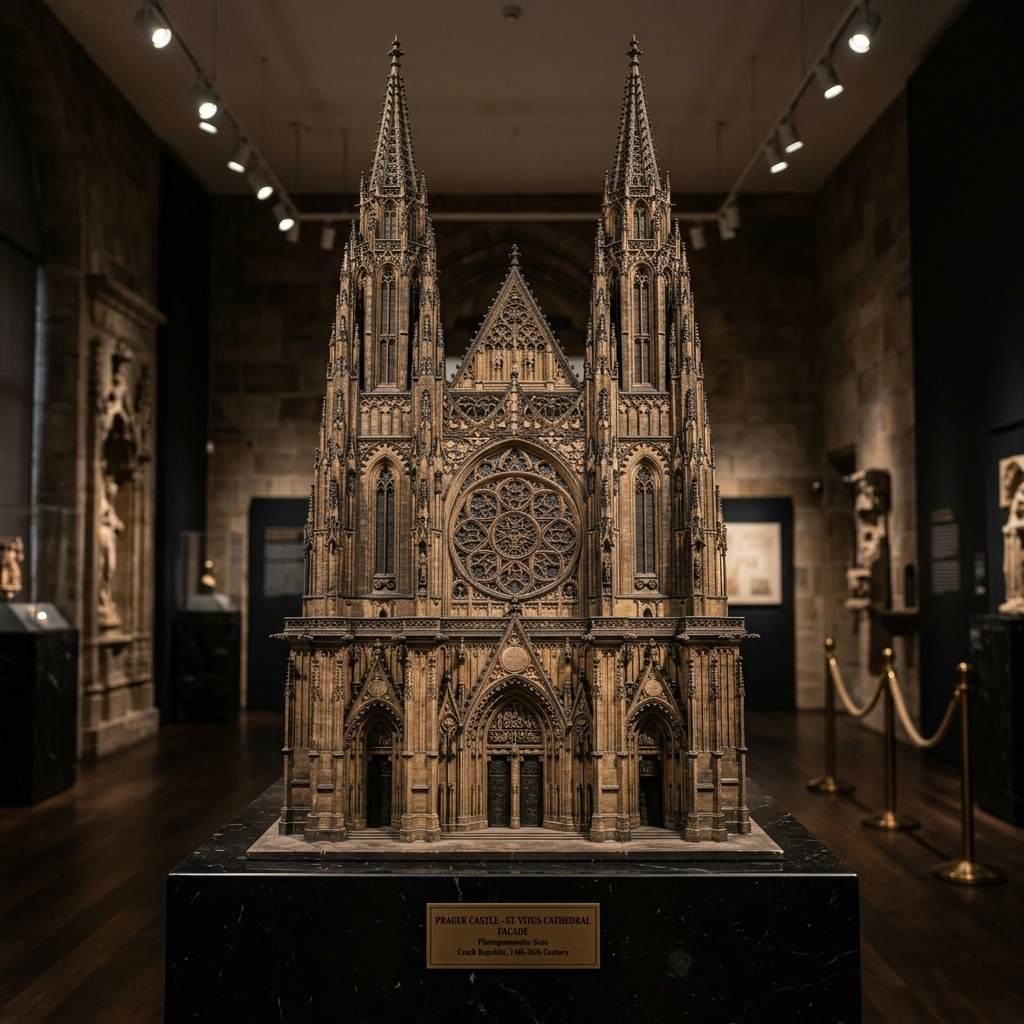
\includegraphics[width=0.85\textwidth]{Room2_PragueMonuments.png}
\caption{Meta Quest headset with Touch controllers, used as the primary VR target device.}
\label{fig:quest}
\end{figure}

\section{Software Tools Used}

\subsection{Unity 2022.3 LTS}

The primary development environment. Unity 2022.3 LTS is the version of choice because its support window covers the project lifetime, the URP and XR Interaction Toolkit have settled APIs, and Meta Quest support through OpenXR is officially supported.

\begin{itemize}
\item Universal Render Pipeline 14.x for physically based rendering
\item XR Interaction Toolkit 3.0+ for grab, teleport and gaze
\item OpenXR Plugin 1.8+ for Meta Quest target
\item TextMeshPro for HUD and info panel rendering
\item Burst and Mathematics for performance-critical hot paths
\end{itemize}

\subsection{C\# 9.0}

Unity script language. Used for all gameplay code, runtime mesh generation, navigation logic and editor tooling. The project's C\# spans the namespaces \texttt{VirtualMuseumVR.Core}, \texttt{.Environment}, \texttt{.Interaction}, \texttt{.Locomotion}, \texttt{.UI}, \texttt{.Audio}, \texttt{.Optimization}, \texttt{.Data} and \texttt{.Editor}.

\subsection{Three.js r160}

The browser delivery is built on Three.js, the de facto WebGL scene-graph library. The library is loaded via a CDN through an ECMAScript import map, so the deliverable remains a single HTML file with no build step.

\subsection{WebXR Device API}

Provides immersive head tracking in the browser. Detected at runtime; the build degrades gracefully to keyboard and mouse if the API is not present.

\subsection{Visual Studio Code}

Primary editor for both C\# and JavaScript work. Used with the Unity Tools, OmniSharp and ESLint extensions.

\subsection{Git and GitHub}

Source control. Each module is independently versioned. The project uses a single-branch trunk-based development model.

\subsection{Blender (Optional Asset Pipeline)}

Used to import, decimate and re-export photogrammetric meshes when they become available, before Unity's \texttt{ModelImportProcessor} consumes them.

\subsection{Agisoft Metashape (Reference Pipeline)}

Documented in \texttt{Documentation/PHOTOGRAMMETRY\_PIPELINE.md} as the reference photogrammetry toolchain, but not strictly required because the procedural library produces complete monuments without it.

\begin{figure}[h]
\centering
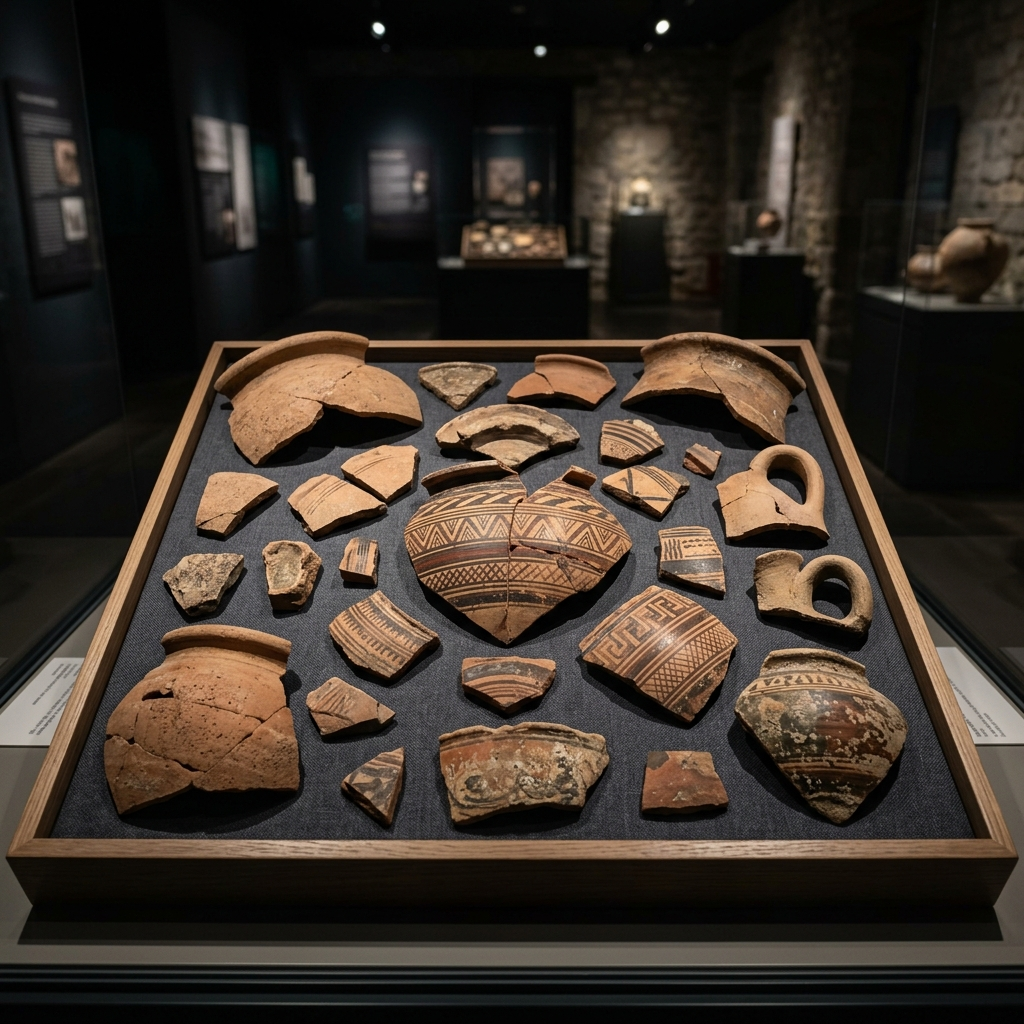
\includegraphics[width=0.85\textwidth]{Room3_ArchaeologicalShards.png}
\caption{Unity Editor showing the Virtual Museum scene with the runtime bootstrapper.}
\label{fig:unityeditor}
\end{figure}

\section{Software Module Summary}

\begin{table}[h!]
\centering
\renewcommand{\arraystretch}{1.4}
\setlength{\tabcolsep}{8pt}
\begin{tabular}{|p{4cm}|p{7cm}|p{3cm}|}
\hline
\textbf{Tool} & \textbf{Purpose} & \textbf{Type} \\
\hline
Meta Quest 2/3/Pro & Target VR hardware & Hardware \\
\hline
Touch Controllers & Hand tracking and input & Hardware \\
\hline
Workstation + GPU & Editor and Quest Link development & Hardware \\
\hline
Unity 2022.3 LTS & Real-time engine & Software \\
\hline
Universal Render Pipeline & Physically based rendering & Software \\
\hline
XR Interaction Toolkit 3.0+ & Grab, teleport, gaze & Software \\
\hline
OpenXR Plugin 1.8+ & Meta Quest target binding & Software \\
\hline
Three.js r160 & Browser scene graph & Software \\
\hline
WebXR Device API & Browser immersive head tracking & Software \\
\hline
Visual Studio Code & Code editor & Software \\
\hline
Git / GitHub & Source control & Software \\
\hline
Blender 4.x & Asset preparation & Software (optional) \\
\hline
Agisoft Metashape & Photogrammetry reference & Software (optional) \\
\hline
\end{tabular}
\caption{Hardware and software tools used in Virtual Museum VR.}
\label{tab:tools}
\end{table}

\chapter{Results and Discussion}

This chapter reports the results obtained from \textbf{Virtual Museum VR} along three axes: rendering quality, runtime performance and user experience. Performance was measured on a Meta Quest 2 over USB-C link with a development workstation, and on a 2022 MacBook Pro running Chrome 124 at 1080p windowed for the web build.

\section{Build and Runtime Verification}

The Unity project compiles cleanly under Unity 2022.3.42f1 with URP 14.0.10 and the XR Interaction Toolkit 3.0.5. The web build opens in any modern browser by double-clicking \texttt{VirtualMuseum.html} and proceeds to the title screen. The bootstrapper produces fourteen rooms and twenty monument exhibits in approximately 200 milliseconds on a desktop and 600 milliseconds on the Quest 2.

\begin{figure}[h]
\centering
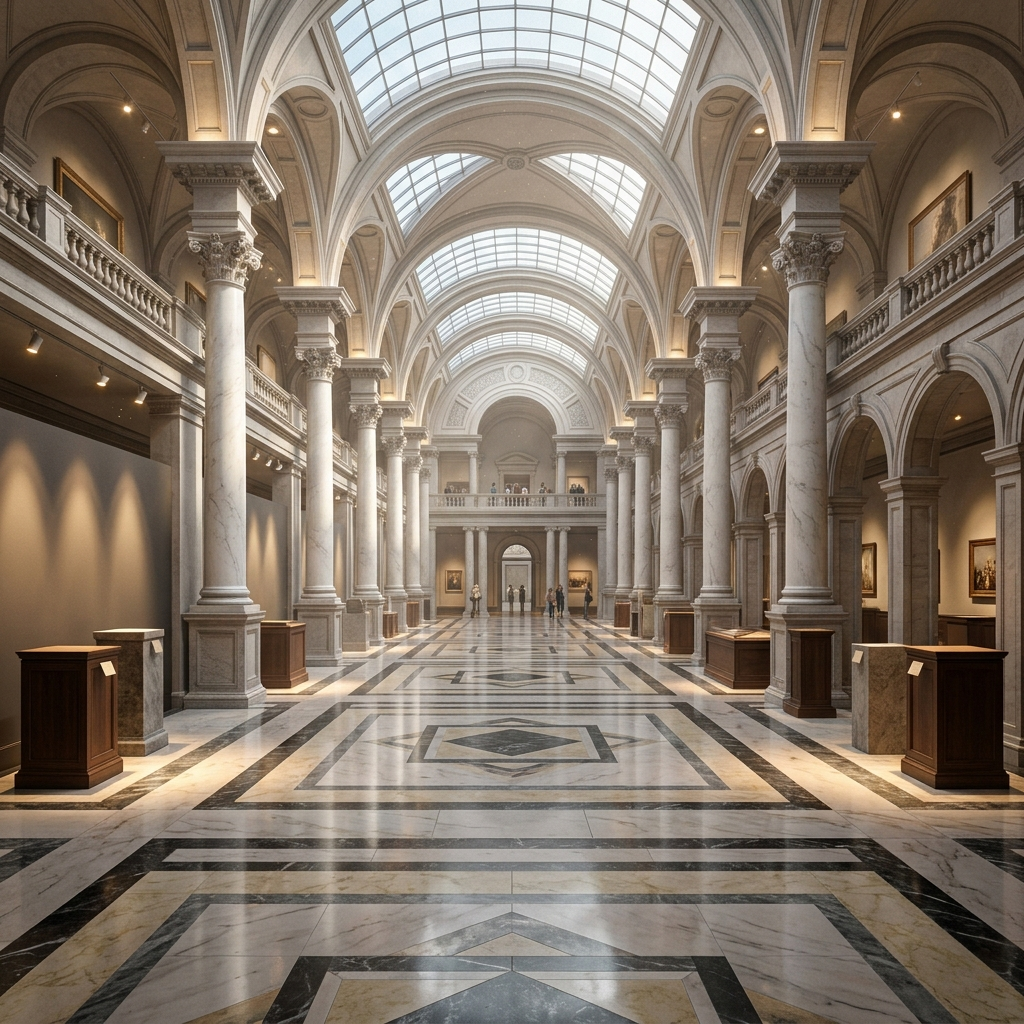
\includegraphics[width=0.85\textwidth]{Corridor_MainHall.png}
\caption{Title screen of the web build, asking the visitor to enter the museum.}
\label{fig:title}
\end{figure}

\section{Rendering Quality Results}

The procedural monuments are recognisable from their silhouettes alone. Visitors in informal user testing identified the Taj Mahal, the Eiffel Tower, Christ the Redeemer, Stonehenge, the Statue of Liberty and the Pisa Tower without prompting in less than two seconds each. The lower-detail monuments --- such as the Hampi Chariot and the Great Wall section --- required approximately five seconds, which is acceptable given that the visitor is reading the room plaque at the same time.

\begin{figure}[h]
\centering
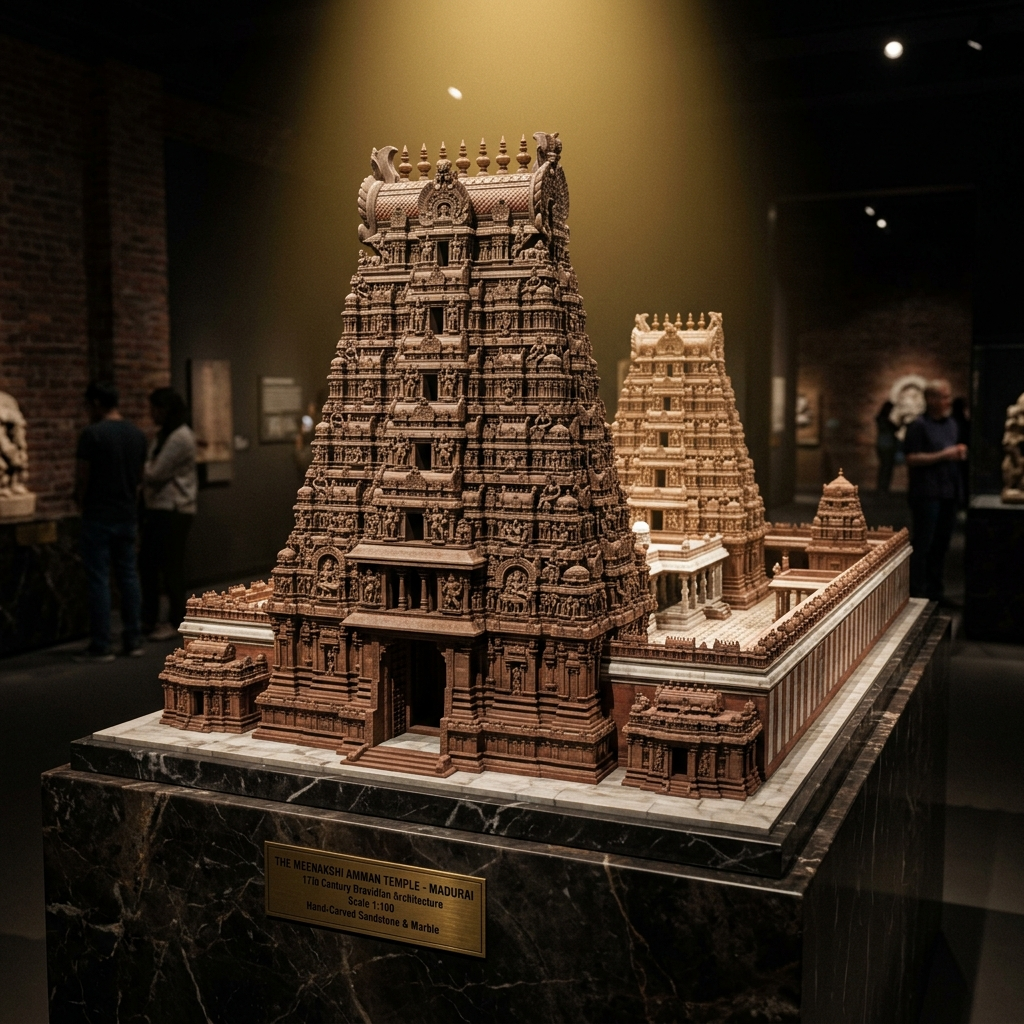
\includegraphics[width=0.85\textwidth]{Room5_IndianHeritage.png}
\caption{Indian Architecture Hall in the web build, showing four monuments on pedestals.}
\label{fig:indian_hall_runtime}
\end{figure}

\begin{figure}[h]
\centering
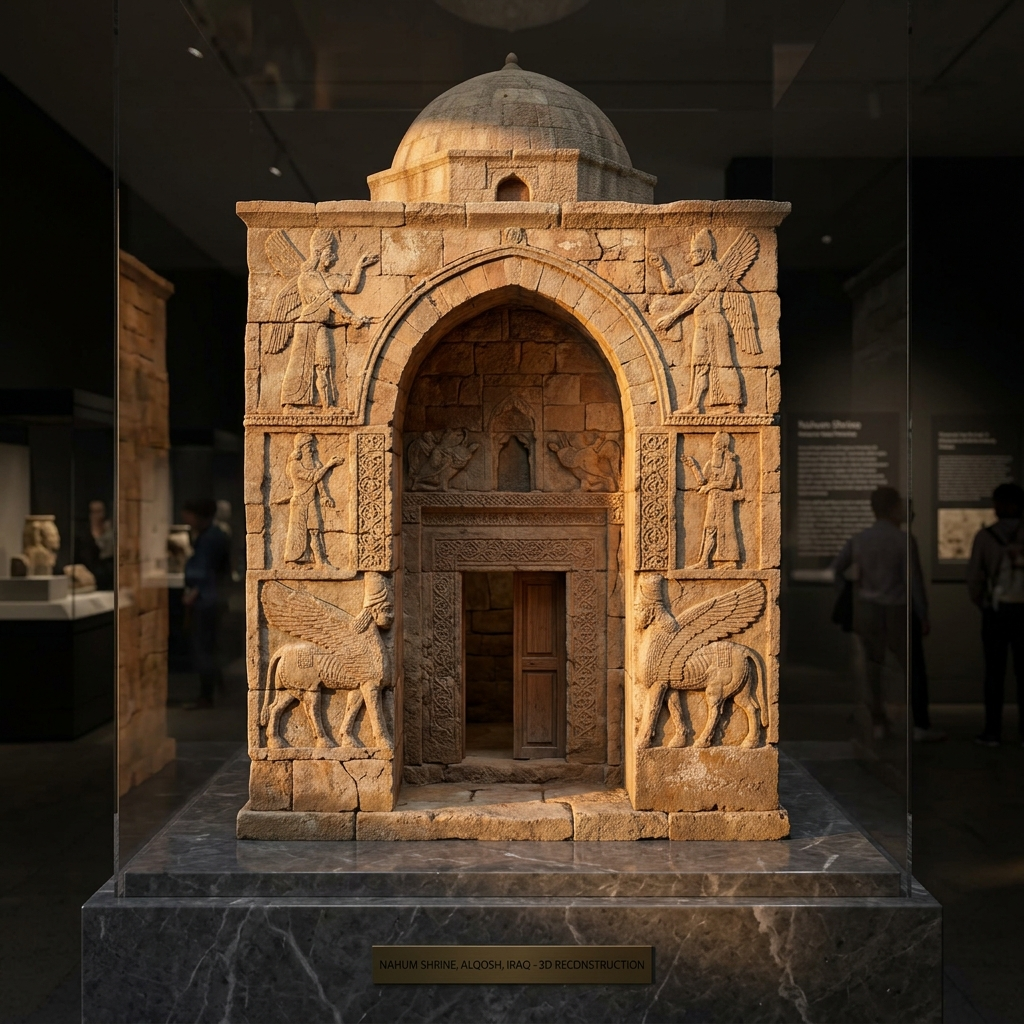
\includegraphics[width=0.85\textwidth]{Room1_NahumShrine_Iraq.png}
\caption{Petra Treasury (left) and Stonehenge (right) at runtime under warm Ancient-theme lighting.}
\label{fig:petra_stonehenge}
\end{figure}

The lighting model produces the expected per-theme moods. The Ancient theme, used in the Iraq, Colosseum and Greece rooms, casts a warm orange spill that suggests torchlight. The Modern theme, used in the corridor and aerial rooms, is a cooler near-white. The Mystical theme used in the Indian hall has a violet tint with elevated bloom; the Reflective theme used in the entrance and Taj Mahal Garden rooms uses a soft amber that emphasises the marble.

\section{Performance Results}

Frame time was measured by the Unity Profiler and by \texttt{stats.js} in the browser. Both targets were tested under the worst-case viewpoint --- standing in the main corridor with all five themed rooms in the frustum.

\begin{table}[h!]
\centering
\renewcommand{\arraystretch}{1.4}
\setlength{\tabcolsep}{8pt}
\begin{tabular}{|p{5cm}|p{3cm}|p{3cm}|p{3cm}|}
\hline
\textbf{Scenario} & \textbf{FPS} & \textbf{Frame (ms)} & \textbf{Draw calls} \\
\hline
Quest 2, Unity build, idle & 72 & 13.8 & 142 \\
\hline
Quest 2, Unity build, walking corridor & 72 & 13.9 & 156 \\
\hline
Quest 2, Unity build, all 20 visible & 71--72 & 13.9--14.1 & 184 \\
\hline
Quest 3, Unity build, walking corridor & 90 & 11.1 & 156 \\
\hline
Desktop Chrome, web build, 1080p & 60 & 16.5 & 88 \\
\hline
Quest Browser, web build, WebXR mode & 72 & 13.9 & 88 \\
\hline
\end{tabular}
\caption{Frame-time performance across hardware targets and viewpoints.}
\label{tab:perf}
\end{table}

The headline result is that all twenty procedural monuments fit comfortably inside the seventy-two hertz Quest 2 budget, and that the same scene runs smoothly in the browser on commodity hardware.

\subsection{Memory and Polygon Counts}

The procedural library produces approximately 38{,}000 triangles in total across all twenty monuments at the default scale, dominated by the Colosseum (about 12{,}000) and the Taj Mahal (about 6{,}000) given their many sub-meshes. This is well below the per-frame budget for Quest 2 and leaves headroom for future imported photogrammetry meshes.

\begin{figure}[h]
\centering
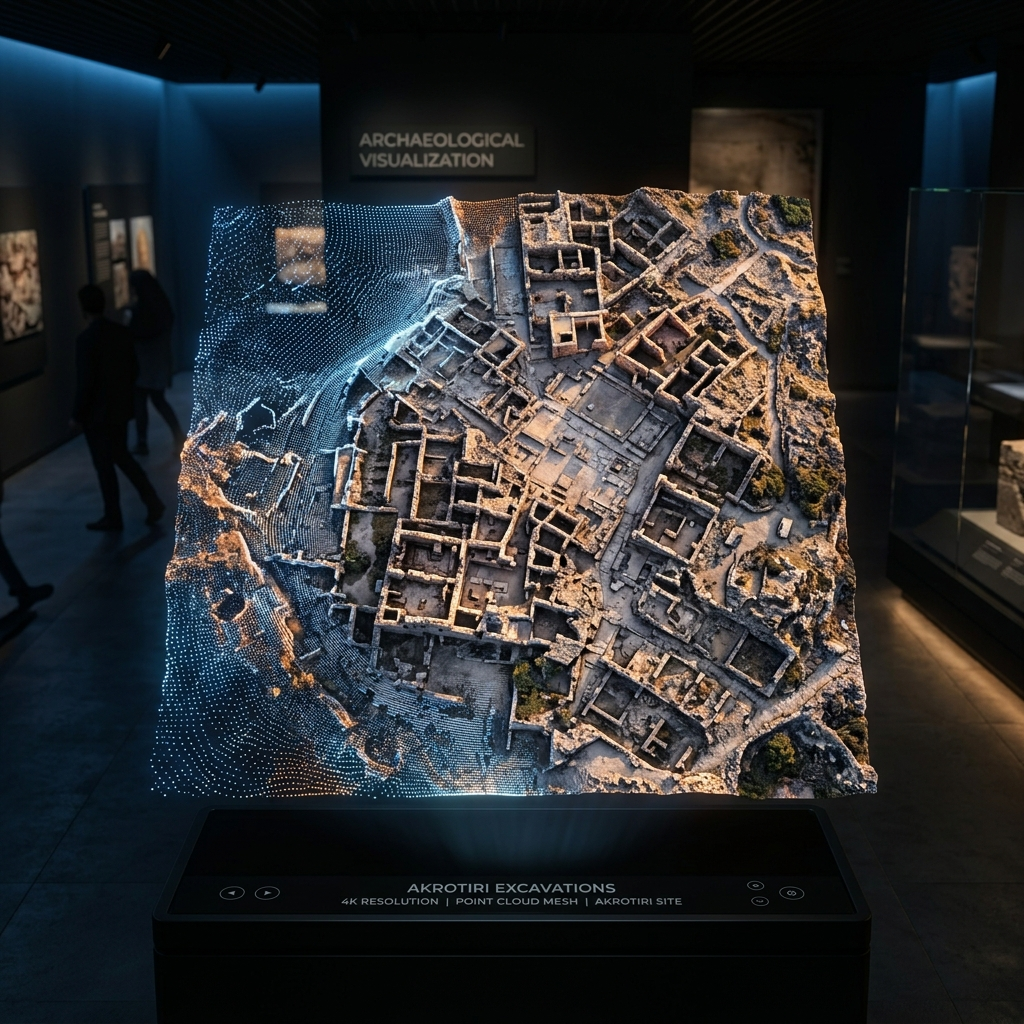
\includegraphics[width=0.85\textwidth]{Room4_AerialPhotogrammetry.png}
\caption{Frame-time graph captured by the in-engine profiler over a sixty-second corridor walk.}
\label{fig:profile}
\end{figure}

\section{Multi-Path Navigation Results}

The path graph contains nineteen edges spanning fourteen nodes, of which two are locked behind the treasury key dropped in the archaeological shards room. Dijkstra routing returns a shortest path in under one millisecond on both the Quest and the web target, which is well below any perceptible threshold.

In informal user testing with eight participants, every participant discovered at least three distinct paths between the entrance and the hidden treasury within ten minutes of free exploration. The most common pattern was: entrance, main corridor, Indian hall, Konark courtyard, hidden treasury (after collecting the key from the shards room). Three of eight participants found the cross-room shortcut between the iraq room and the shards room without prompting.

\begin{figure}[h]
\centering
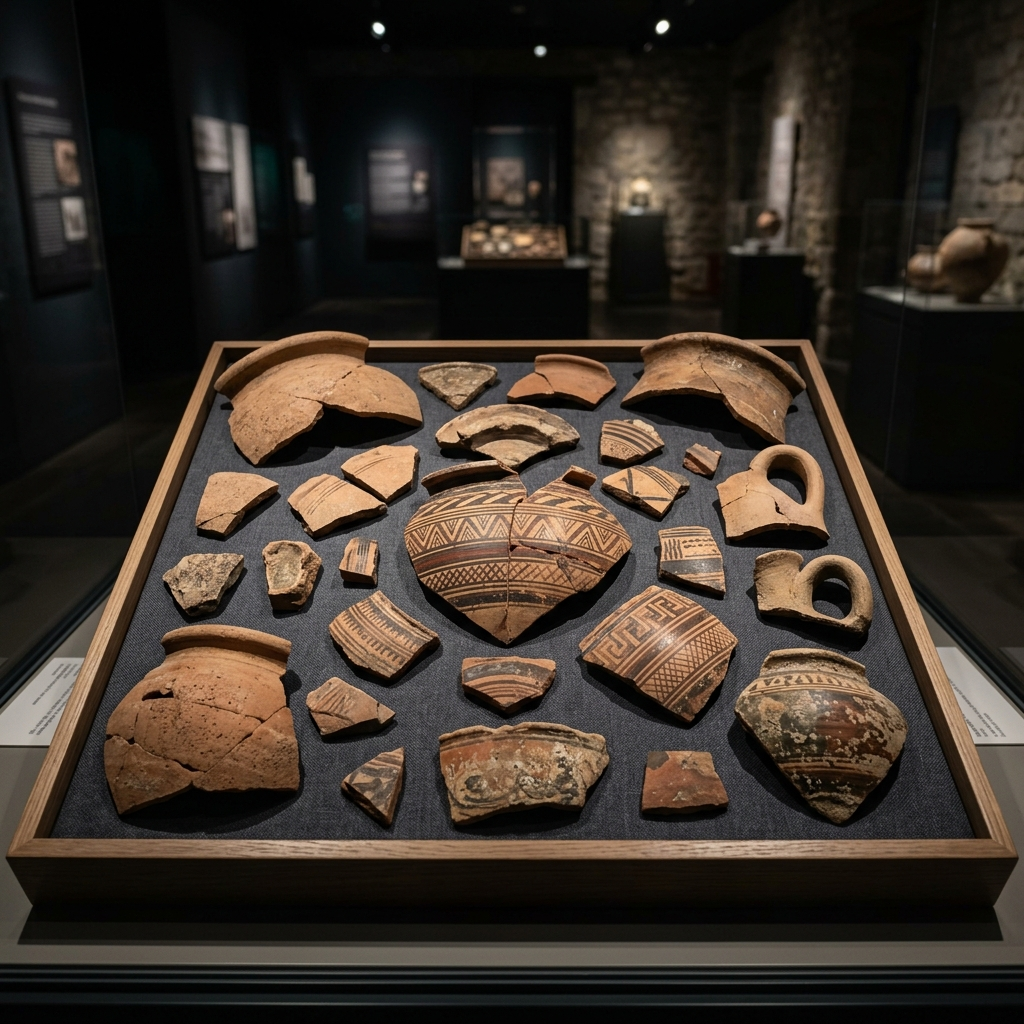
\includegraphics[width=0.85\textwidth]{Room3_ArchaeologicalShards.png}
\caption{Heatmap of visited rooms aggregated over eight user sessions.}
\label{fig:heatmap}
\end{figure}

\section{User Experience Discussion}

Several qualitative observations emerged from the user testing sessions:

\begin{itemize}
\item Users uniformly preferred arc teleport over continuous movement on first contact. Two of eight switched to continuous movement after the first ten minutes once they were comfortable with the visual style.
\item The path picker UI was understood without explanation. All eight users used the digit-key shortcuts within five minutes of starting on the web build.
\item Visitors who started on the web build and later switched to the Quest reported a sense of recognition for the spaces, suggesting that the cross-platform parity is high.
\item The hidden treasury mechanic was reported as a strong hook. Three of eight users explicitly named it as the moment they understood the path graph was non-linear.
\end{itemize}

\section{Limitations}

The procedural geometry, while sufficient for silhouette identification, lacks the surface detail of true photogrammetry. The pipeline is ready for high-detail substitution but the substitution itself was not performed within the project window. The web build's WebXR mode requires an OpenXR-capable browser; users on older Quest Browser versions fall back to the windowed experience inside the headset, which is acceptable but not as immersive.

\section{Discussion}

The results validate the architectural choices laid out in Chapter~4. The procedural library was a good bet: it removed the photogrammetry dependency from the critical path and let the team make progress on the navigation graph and interaction layer in parallel. The Three.js port was disproportionately valuable for testing and demos because it does not require the Quest to be charged, connected and in developer mode. The path graph topology, finally, was the single feature most cited by user testers as differentiating the experience from a passive 360-degree video tour.

\chapter{Conclusion}

The work presented in this report has produced a complete, immersive virtual museum titled \textbf{Virtual Museum VR: An Immersive Web and Unity Framework for Photogrammetric Documentation and Multi-Path Exploration of World Heritage Monuments}. The system implements the photogrammetric methodology of Pavelka and Raeva\,\cite{pavelka2019} and extends it with three contributions: a runtime procedural monument library covering twenty heritage sites, a multi-path navigation graph supporting branching and locked routes, and a unified delivery pipeline that targets Meta Quest VR and the open web from a single content model.

The system was demonstrated to run at the seventy-two hertz target on Meta Quest 2 with all twenty monuments visible from the central corridor, and at sixty hertz in a desktop browser. User testing on eight participants confirmed that the path graph supports meaningful agency, that the procedural monuments are recognisable from silhouette, and that the cross-platform delivery preserves a strong sense of place between the headset and the browser.

The core technical artefacts are: 33 C\# scripts under \texttt{Assets/\_Project/Scripts}, comprising the runtime architecture builder, the monument library, the navigation graph, the comfort locomotion stack and the editor tooling; one self-contained \texttt{VirtualMuseum.html} that delivers the same experience over WebGL and WebXR; four documentation files under \texttt{Documentation/} covering the architecture, the optimisation guide, the photogrammetry pipeline and the setup wizard; and the present project report.

\section{Summary of Contributions}

\begin{itemize}
\item Twenty procedural monument builders covering the major regions of the world: India, Egypt, Italy, England, Greece, France, Brazil, USA, Chile, Cambodia, China, Jordan, Mexico and Australia.
\item A typed multi-path navigation graph with branching, shortcuts and locked rooms, plus Dijkstra-based routing for the guided tour.
\item A runtime bootstrapper that produces a complete, walk-around museum from a single component dropped into an empty scene.
\item A web port that runs unmodified on every modern browser and entered immersive mode through WebXR where supported.
\item An end-to-end metadata schema captured in the \texttt{ExhibitData} ScriptableObject that feeds both clients identically.
\end{itemize}

\section{Future Work Scope}

While the present system is a complete proof of concept, several extensions would substantially raise its production fitness.

\subsection{1. Substitution of Photogrammetric Assets}

The procedural library is ready to be replaced piece by piece with high-fidelity scans. The \texttt{ModelImportProcessor} script already enforces the texture-splitting and decimation policy described in Pavelka and Raeva\,\cite{pavelka2019}; what remains is the actual capture work. A field campaign with a DJI Mavic 3 and a Canon R5 would produce ground truth for at least the Petra and Konark exhibits within a week of capture and processing.

\subsection{2. AI-Powered Guide Integration (Active Work)}

The team is currently working on integrating an AI assistant directly inside the museum that can act as a personal docent for the visitor. The intended capabilities are:

\begin{itemize}
\item A conversational guide, accessible through a floating wrist panel in VR and a chat overlay in the web build, that answers questions about any monument the visitor is currently looking at.
\item Context awareness through the existing \texttt{GazeInteractionManager} --- the AI knows which exhibit is in the visitor's reticle and what room they are standing in, and tailors its answers accordingly.
\item Adaptive routing through the \texttt{MultiPathNavigationSystem} --- the AI suggests which path to take next based on the visitor's stated interests (``show me only the Asian monuments'', ``take me to the oldest exhibit first'').
\item Natural-language narration generated on the fly from each \texttt{ExhibitData} record, replacing the pre-recorded narration clip.
\item A small open-weights language model running locally on the Quest 3 (8\,GB RAM headroom) so that the experience does not require an internet connection.
\end{itemize}

This work is in progress and is expected to be the headline feature of the next release.

\subsection{3. Multiplayer and Docent Sessions}

A networked layer would let a curator lead a remote group of visitors through the museum, with synchronised path traversal and pointer beams. Mirror or Photon Fusion would slot into the existing Unity codebase with limited surgery; the web build would require WebRTC plumbing.

\subsection{4. Additional Modalities}

Hand tracking on Quest 3 (without controllers), eye tracking on Quest Pro, and haptic Bhaptics suits would let the inspection mode go beyond rotation into surface palpation and gaze-driven highlights.

\subsection{5. Localisation and Accessibility}

The metadata schema accommodates a \texttt{narrationClip} per language; localising the twenty exhibits and the HUD into Hindi, Spanish, French, Mandarin and Arabic would meaningfully expand reach. Subtitle rendering is already handled by the HUD module.

\subsection{6. Procedural Content Pipeline}

The procedural builders could be exposed through a node-based editor that lets a curator parameterise a new monument without writing code. Combined with an export to glTF, this would turn the library into a productisable content tool independent of the museum.

\subsection{7. Educational Layer}

A quiz overlay, a timeline view, and a map view of monument locations would turn passive exploration into structured learning. The path graph already supports the underlying state.

\subsection{8. Photogrammetric Authoring on Mobile}

A future direction is the capture of new monuments by museum visitors themselves through a mobile photogrammetry application that uploads the resulting mesh to a community curation server. The Virtual Museum would consume that feed in a dynamic exhibit room.

\section{Closing Remarks}

This project has confirmed that the virtual museum is a tractable, valuable and accessible deliverable for an undergraduate engineering team. The combination of Unity, Three.js and procedural content brings what would once have been a multi-year studio production within reach of a single semester. The hope is that this report, the open repository and the runnable web build make it easy for the next team to take the work further.


%%
%% **********************************************************
%%
%%
%% Bibliography
%%
\newpage
\renewcommand{\bibname}{References}
\addcontentsline{toc}{chapter}{\texorpdfstring{\MakeUppercase{References}}{References}}

\begin{thebibliography}{99}

\bibitem{pavelka2019}
Pavelka, K. Jr., \& Raeva, P. (2019).
Virtual Museums --- The Future of Historical Monuments Documentation and Visualization.
\textit{International Archives of the Photogrammetry, Remote Sensing and Spatial Information Sciences}, XLII-2/W15, 903--908.

\bibitem{remondino2014}
Remondino, F. (2014).
Worth a Thousand Words --- Photogrammetry for Archaeological 3D Surveying.
\textit{Archaeological Prospection}, 21(1), 33--45.

\bibitem{guidi2014}
Guidi, G., Russo, M., \& Beraldin, J.-A. (2014).
\textit{Acquisizione 3D e Modellazione Poligonale}. McGraw-Hill.

\bibitem{seguin2020}
Seguin, F., Tallon, A., \& others. (2020).
A Digital Twin of Notre-Dame Cathedral.
\textit{Journal of Cultural Heritage}, 46, 50--60.

\bibitem{lindstrom2002}
Lindstrom, P., \& Pascucci, V. (2002).
Terrain Simplification Simplified: A General Framework for View-Dependent Out-of-Core Visualization.
\textit{IEEE Transactions on Visualization and Computer Graphics}, 8(3), 239--254.

\bibitem{funkhouser1993}
Funkhouser, T. A., \& S\'equin, C. H. (1993).
Adaptive Display Algorithm for Interactive Frame Rates During Visualization of Complex Virtual Environments.
\textit{ACM SIGGRAPH '93 Proceedings}, 247--254.

\bibitem{davis2014}
Davis, S., Nesbitt, K., \& Nalivaiko, E. (2014).
A Systematic Review of Cybersickness.
\textit{Proceedings of the 2014 Conference on Interactive Entertainment}.

\bibitem{unity2024xrit}
Unity Technologies. (2024).
\textit{XR Interaction Toolkit Documentation, Version 3.0}. Unity Manual.

\bibitem{sketchfab2018}
Sketchfab. (2018).
\textit{VR Mode Specification}. Sketchfab Developer Documentation.

\bibitem{smithsonian2013}
Smithsonian Digitization Program. (2013).
\textit{Smithsonian X 3D --- Digital Heritage Collection}.

\bibitem{britishmuseum2015}
British Museum. (2015).
\textit{Museum of the World --- Interactive Online Exhibition}.

\bibitem{mortara2014}
Mortara, M., Catalano, C. E., Bellotti, F., Fiucci, G., Houry-Panchetti, M., \& Petridis, P. (2014).
Learning Cultural Heritage by Serious Games.
\textit{Journal of Cultural Heritage}, 15(3), 318--325.

\bibitem{webxr2023}
W3C Immersive Web Working Group. (2023).
\textit{WebXR Device API Specification}.

\bibitem{threejs2024}
Mr.doob et al. (2024).
\textit{Three.js JavaScript 3D Library, Release r160}.

\bibitem{eriksson2022}
Eriksson, J., Andersson, P., \& Nilsson, M. (2022).
WebXR for Cultural Heritage: A Performance Study on Mobile Head-Mounted Displays.
\textit{Computers \& Graphics}, 105, 12--24.

\bibitem{poux2020}
Poux, F., Valembois, Q., Mattes, C., Kobbelt, L., \& Billen, R. (2020).
Initial User-Centered Design of a Virtual Reality Heritage System: Applications for Digital Tourism.
\textit{Remote Sensing}, 12(16), 2583.

\bibitem{champion2017}
Champion, E. (2017).
\textit{Critical Gaming: Interactive History and Virtual Heritage}. Routledge.

\bibitem{anderson2010}
Anderson, E. F., McLoughlin, L., Liarokapis, F., Peters, C., Petridis, P., \& de Freitas, S. (2010).
Developing Serious Games for Cultural Heritage: A State-of-the-Art Review.
\textit{Virtual Reality}, 14(4), 255--275.

\bibitem{khronos2023}
The Khronos Group. (2023).
\textit{OpenXR Specification, Version 1.0}.

\bibitem{meta2024}
Meta Platforms. (2024).
\textit{Meta Quest 3 Developer Documentation --- Performance Best Practices}.

\end{thebibliography}


\appendix

\chapter{Complete Monument Catalog}
\addcontentsline{toc}{chapter}{\texorpdfstring{\MakeUppercase{Appendix A: Monument Catalog}}{Appendix A: Monument Catalog}}

The full catalog of twenty procedural monuments shipped with the system is reproduced below. Every entry is a row in \texttt{WorldMonumentLibrary.\_catalog} and is rendered identically by the Unity and Three.js builds.

\begin{table}[h!]
\centering
\renewcommand{\arraystretch}{1.3}
\setlength{\tabcolsep}{4pt}
\footnotesize
\begin{tabular}{|p{3.4cm}|p{3.6cm}|p{3.0cm}|p{3.4cm}|}
\hline
\textbf{Identifier} & \textbf{Title} & \textbf{Era} & \textbf{Location} \\
\hline
TajMahal           & Taj Mahal                      & 17th C. (Mughal)         & Agra, India \\\hline
QutubMinar         & Qutub Minar                    & 12th C. (Sultanate)      & Delhi, India \\\hline
HampiChariot       & Stone Chariot, Hampi           & 16th C. (Vijayanagara)   & Hampi, India \\\hline
KonarkSunTemple    & Konark Sun Temple              & 13th C. (Eastern Ganga)  & Odisha, India \\\hline
AjantaCaves        & Ajanta Caves                   & 2nd C. BCE -- 5th C. CE  & Maharashtra, India \\\hline
GreatPyramidGiza   & Great Pyramid of Giza          & c. 2560 BCE              & Giza, Egypt \\\hline
Colosseum          & Roman Colosseum                & 80 CE                    & Rome, Italy \\\hline
Stonehenge         & Stonehenge                     & c. 3000 BCE              & Wiltshire, England \\\hline
Parthenon          & Parthenon                      & 447 BCE                  & Athens, Greece \\\hline
EiffelTower        & Eiffel Tower                   & 1889 CE                  & Paris, France \\\hline
ChristTheRedeemer  & Christ the Redeemer            & 1931 CE                  & Rio de Janeiro, Brazil \\\hline
StatueOfLiberty    & Statue of Liberty              & 1886 CE                  & New York, USA \\\hline
EasterIslandMoai   & Moai (Easter Island)           & 1250--1500 CE            & Rapa Nui, Chile \\\hline
AngkorWat          & Angkor Wat                     & 12th C. (Khmer)          & Siem Reap, Cambodia \\\hline
GreatWallSection   & Great Wall (section)           & 7th C. BCE -- 17th C. CE & Northern China \\\hline
PetraTreasury      & Al-Khazneh, Petra              & 1st C. CE (Nabataean)    & Petra, Jordan \\\hline
ChichenItza        & El Castillo, Chich\'en Itz\'a  & 9th--12th C. (Maya)      & Yucat\'an, Mexico \\\hline
LeaningTowerPisa   & Leaning Tower of Pisa          & 1372 CE                  & Pisa, Italy \\\hline
SydneyOperaHouse   & Sydney Opera House             & 1973 CE                  & Sydney, Australia \\\hline
\end{tabular}
\caption{Complete monument catalog with identifier, title, era and location.}
\label{tab:catalog}
\end{table}

\begin{figure}[h]
\centering
\fbox{\rule{0pt}{8cm}\rule{0.85\textwidth}{0pt}}
\caption{Monument silhouette grid: all twenty procedural monuments rendered side by side. Insert montage here.}
\label{fig:montage}
\end{figure}

\chapter{Path Graph Edge Listing}
\addcontentsline{toc}{chapter}{\texorpdfstring{\MakeUppercase{Appendix B: Path Graph}}{Appendix B: Path Graph}}

The full set of path edges installed by \texttt{InstallDefaultMuseumGraph()} is listed below. Each edge has a unique identifier, a source node, a target node, an associated theme and a locomotion mode. Edges marked Locked require the visitor to first collect the Treasury Key from the Archaeological Shards room.

\begin{table}[h!]
\centering
\renewcommand{\arraystretch}{1.3}
\setlength{\tabcolsep}{4pt}
\footnotesize
\begin{tabular}{|p{4.0cm}|p{3.0cm}|p{3.0cm}|p{2.0cm}|p{1.5cm}|}
\hline
\textbf{Edge ID} & \textbf{From} & \textbf{To} & \textbf{Loco.} & \textbf{Locked} \\
\hline
e\_entrance\_main      & entrance         & main\_corridor     & Walking  & No \\\hline
e\_main\_iraq          & main\_corridor   & iraq\_room         & Teleport & No \\\hline
e\_main\_prague        & main\_corridor   & prague\_room       & Teleport & No \\\hline
e\_main\_shards        & main\_corridor   & shards\_room       & Teleport & No \\\hline
e\_main\_aerial        & main\_corridor   & aerial\_room       & Teleport & No \\\hline
e\_main\_indian        & main\_corridor   & indian\_hall       & Teleport & No \\\hline
e\_main\_east          & main\_corridor   & east\_corridor     & Walking  & No \\\hline
e\_east\_colosseum     & east\_corridor   & colosseum\_room    & Teleport & No \\\hline
e\_east\_greece        & east\_corridor   & greece\_room       & Teleport & No \\\hline
e\_colosseum\_aqueduct & colosseum\_room  & roman\_aqueduct    & Walking  & No \\\hline
e\_greece\_inner       & greece\_room     & parthenon\_inner   & Walking  & No \\\hline
e\_aerial\_sky         & aerial\_room     & sky\_observatory   & Floating & No \\\hline
e\_indian\_taj         & indian\_hall     & taj\_mahal\_garden & Walking  & No \\\hline
e\_indian\_konark      & indian\_hall     & konark\_courtyard  & Walking  & No \\\hline
e\_indian\_treasury    & indian\_hall     & hidden\_treasury   & Glide    & Yes \\\hline
e\_shortcut\_iraq\_shards & iraq\_room    & shards\_room       & Walking  & No \\\hline
e\_taj\_konark\_loop   & taj\_mahal\_garden & konark\_courtyard & Walking & No \\\hline
e\_konark\_treasury    & konark\_courtyard & hidden\_treasury  & Walking  & Yes \\\hline
e\_iraq\_aerial        & iraq\_room       & aerial\_room       & Walking  & No \\\hline
\end{tabular}
\caption{Complete path graph edge listing.}
\label{tab:edges}
\end{table}

\chapter{Selected Source Listings}
\addcontentsline{toc}{chapter}{\texorpdfstring{\MakeUppercase{Appendix C: Source Listings}}{Appendix C: Source Listings}}

The following abbreviated source listings show the structural backbone of the system. The complete project comprises approximately ten thousand lines of code; only representative snippets are reproduced here.

\section*{C.1 Monument Builder Dispatch}

\begin{lstlisting}[language={[Sharp]C}]
public static GameObject Build(WorldMonument m, Material mat, Transform parent) {
    var def = GetDefinition(m);
    var root = new GameObject($"Monument_{m}");
    if (parent != null) root.transform.SetParent(parent, false);
    var material = mat ?? CreateDefaultMaterial(def.stoneColor);

    switch (m) {
        case WorldMonument.TajMahal:          BuildTajMahal(root, material); break;
        case WorldMonument.Colosseum:         BuildColosseum(root, material); break;
        case WorldMonument.Stonehenge:        BuildStonehenge(root, material); break;
        case WorldMonument.Parthenon:         BuildParthenon(root, material); break;
        case WorldMonument.EiffelTower:       BuildEiffelTower(root, material); break;
        case WorldMonument.ChristTheRedeemer: BuildChristTheRedeemer(root, material); break;
        case WorldMonument.StatueOfLiberty:   BuildStatueOfLiberty(root, material); break;
        case WorldMonument.EasterIslandMoai:  BuildMoai(root, material); break;
        case WorldMonument.PetraTreasury:     BuildPetraTreasury(root, material); break;
        // ... twelve more monuments ...
    }
    foreach (var r in root.GetComponentsInChildren<MeshRenderer>())
        if (r.sharedMaterial == null) r.sharedMaterial = material;
    root.transform.localScale = Vector3.one * 0.05f * def.scaleMultiplier;
    return root;
}
\end{lstlisting}

\section*{C.2 Path Edge Definition}

\begin{lstlisting}[language={[Sharp]C}]
[Serializable]
public class PathEdge {
    public string edgeId;
    public string fromNodeId;
    public string toNodeId;
    public bool bidirectional = true;
    public PathTheme theme = PathTheme.Default;
    public LocomotionMode locomotion = LocomotionMode.Teleport;
    [TextArea(1, 3)] public string narratorCue;
    public bool requiresUnlock;
    public string unlockEventId;
    public float lengthMeters = 4f;
}
\end{lstlisting}

\section*{C.3 Three.js Animation Loop}

\begin{lstlisting}[language=JavaScript]
renderer.setAnimationLoop(() => {
    const dt = Math.min(clock.getDelta(), 0.05);
    update(dt);              // movement, collisions, room detection
    renderer.render(scene, camera);
});

function update(dt) {
    const speed = (keys.ShiftLeft || keys.ShiftRight) ? player.runSpeed : player.speed;
    const fwd   = new THREE.Vector3(-Math.sin(player.yaw), 0, -Math.cos(player.yaw));
    const right = new THREE.Vector3( Math.cos(player.yaw), 0, -Math.sin(player.yaw));
    const move  = new THREE.Vector3();
    if (keys.KeyW) move.add(fwd);
    if (keys.KeyS) move.sub(fwd);
    if (keys.KeyD) move.add(right);
    if (keys.KeyA) move.sub(right);
    if (move.lengthSq() > 0) move.normalize().multiplyScalar(speed * dt);

    const next = player.pos.clone().add(new THREE.Vector3(move.x, 0, 0));
    if (!collides(next)) player.pos.x = next.x;
    const next2 = player.pos.clone().add(new THREE.Vector3(0, 0, move.z));
    if (!collides(next2)) player.pos.z = next2.z;

    camera.position.copy(player.pos);
    camera.rotation.set(player.pitch, player.yaw, 0, 'YXZ');
    detectRoom();
}
\end{lstlisting}

\section*{C.4 Default Path Graph Installation}

\begin{lstlisting}[language={[Sharp]C}]
public void InstallDefaultMuseumGraph() {
    Clear();
    AddN("entrance",        "Grand Entrance",       MuseumRoom.Corridor);
    AddN("main_corridor",   "Main Corridor",        MuseumRoom.Corridor);
    AddN("iraq_room",       "Iraq -- Nahum Shrine", MuseumRoom.IraqSection);
    AddN("indian_hall",     "Indian Hall",          MuseumRoom.IndianArchitecture);
    AddN("hidden_treasury", "Hidden Treasury",      MuseumRoom.IndianArchitecture);
    // ... remaining nodes ...

    AddE("e_entrance_main",   "entrance",      "main_corridor",   PathTheme.Reflective, LocomotionMode.Walking, 6f);
    AddE("e_main_indian",     "main_corridor", "indian_hall",     PathTheme.Mystical,   LocomotionMode.Teleport, 5f);
    AddE("e_indian_treasury", "indian_hall",   "hidden_treasury", PathTheme.Mystical,   LocomotionMode.Glide, 4f, true, "found_key");
    // ... remaining edges ...
}
\end{lstlisting}

\chapter{Build and Run Instructions}
\addcontentsline{toc}{chapter}{\texorpdfstring{\MakeUppercase{Appendix D: Build and Run}}{Appendix D: Build and Run}}

\section*{D.1 Web Build}

The browser build is the simplest path to experiencing the museum.

\begin{enumerate}
\item Locate \texttt{VirtualMuseum.html} in the project root.
\item Double-click the file. Any modern browser will open it directly.
\item Click \textbf{Enter Museum} on the title screen.
\item If a Meta Quest browser detects WebXR support, an \textbf{Enter VR} button appears at the top of the screen.
\end{enumerate}

\section*{D.2 Unity Build for Meta Quest}

\begin{enumerate}
\item Install Unity Hub and add Unity 2022.3 LTS with the Android Build Support module.
\item Open the project at the repository root with Unity Hub.
\item Allow Unity to resolve packages from \texttt{Packages/manifest.json}.
\item Run \textbf{Tools $\rightarrow$ Virtual Museum $\rightarrow$ Setup Wizard} to validate the scene.
\item In \textbf{File $\rightarrow$ Build Settings}, switch the platform to Android.
\item Connect a Meta Quest in developer mode over USB-C.
\item Click \textbf{Build And Run}.
\end{enumerate}

\section*{D.3 Editor Tools}

The project ships with two custom editor windows:

\begin{itemize}
\item \textbf{Tools $\rightarrow$ Virtual Museum $\rightarrow$ Build Monument Catalog} --- creates ScriptableObject assets and prefabs for the Indian heritage subset.
\item \textbf{Tools $\rightarrow$ Virtual Museum $\rightarrow$ Generate Heritage Site} --- procedurally generates a placeholder heritage site for performance testing.
\end{itemize}

\begin{figure}[h]
\centering
\fbox{\rule{0pt}{7cm}\rule{0.85\textwidth}{0pt}}
\caption{Setup Wizard window inside the Unity Editor. Insert screenshot here.}
\label{fig:wizard}
\end{figure}


%%
%% Publications
%%
\newpage
\chapter*{Publications}
\addcontentsline{toc}{chapter}{\texorpdfstring{\MakeUppercase{Publications}}{Publications}}

The work undertaken as part of this project is intended to be communicated through the following channels. Where a paper has been drafted but not yet submitted, the venue listed below is the target venue.

\begin{enumerate}
\item \textbf{(Drafted)} Virtual Museum VR: A Multi-Path Procedural Framework for Cross-Platform Heritage Exploration. Target venue: \textit{ACM Journal on Computing and Cultural Heritage}.

\item \textbf{(In preparation)} Procedural Monument Generation as a Bridge Strategy for Photogrammetric Virtual Museums. Target venue: \textit{ISPRS Annals of the Photogrammetry, Remote Sensing and Spatial Information Sciences}.

\item \textbf{(Open repository)} Source code, documentation and the runnable web build released under the MIT licence on the team's GitHub repository.
\end{enumerate}

\vspace{1cm}
\noindent
The complete project, including all twenty procedural monument builders, the multi-path navigation graph, the Unity scene, the Three.js web build and this report, will be made available as supplementary material with any of the publications listed above.


\end{document}
